\documentclass[11pt,a4paper]{article}

\usepackage[margin=0.85in]{geometry}
\usepackage[T1]{fontenc}
\usepackage[utf8]{inputenc}
\usepackage{amsmath,amssymb,bm}
\usepackage{graphicx}
\usepackage{booktabs}
\usepackage{multirow}
\usepackage{array}
\usepackage{xcolor}
\usepackage{tikz}
\usetikzlibrary{positioning,fit,backgrounds,calc,shapes.geometric}
\usepackage{algorithm}
\usepackage{algorithmic}
\usepackage{caption}
\usepackage{cite}
\usepackage{microtype}
\usepackage[section]{placeins}
\usepackage{hyperref}

\emergencystretch=1.5em

\renewcommand{\topfraction}{0.92}
\renewcommand{\bottomfraction}{0.85}
\renewcommand{\textfraction}{0.07}
\renewcommand{\floatpagefraction}{0.75}
\setcounter{topnumber}{4}
\setcounter{bottomnumber}{4}
\setcounter{totalnumber}{8}

\hypersetup{
  colorlinks=true,
  linkcolor=blue!60!black,
  citecolor=blue!60!black,
  urlcolor=blue!60!black
}

\title{\large\textbf{MEWC-Flow: Modular Elastic Weight Consolidation with Physics-Only Contrastive Regime Routing for Continual Learning of Fluid Flow Surrogates across Reynolds Regimes}}
\date{}

\begin{document}
\maketitle

\bigskip

% ==============================================================================
\section{Motivation \& Research Questions (RQ1--RQ5)}
% ==============================================================================

Neural operators, most notably the Fourier Neural Operator (FNO)~\cite{li2021fno}, accelerate PDE surrogate inference by orders of magnitude, yet suffer severe \textbf{catastrophic forgetting}~\cite{kirkpatrick2017ewc} when deployed across non-stationary flow streams where Reynolds number $Re = U_{\infty} D / \nu$ increases across laminar, supercritical vortex-shedding, transitional, and turbulent regimes~\cite{shi2026striding,winkler2026nfl}. Prior continual operator methods such as SLE-FNO~\cite{elhadidy2026slefno}, Replay-TS~\cite{hemati2026replayts}, and Transolver replay~\cite{wang2026replay}, as well as Reynolds-conditioned models~\cite{guo2026renanet} and autoencoder routers~\cite{ji2026pmoe,kim2026mgann} (Table~\ref{tab:positioning}), leave three critical gaps: (1) task-agnostic routing without leaking privileged $Re$ metadata, (2) complex-valued Fisher consolidation for spectral weights (\texttt{torch.cfloat}), and (3) leak-free physical and multi-step rollout evaluation. Extending our prior MEWC-RL++ framework~\cite{hasan2026mewcrlpp}, we answer five research questions:

\begin{itemize}
  \item \textbf{RQ1 (Stability--Plasticity Across Regimes):} How effectively do modular regime adapters combined with complex-parameter Adaptive EWC (A-EWC) and matched-budget episodic replay prevent catastrophic forgetting while preserving plasticity across sequential Reynolds-number shifts, including genuine hydrodynamic bifurcations?
  \item \textbf{RQ2 (Physical Consistency \& Rollout Fidelity):} Beyond single-step pixel MSE, does MEWC-Flow preserve physical invariants (vorticity RMSE, divergence-free incompressibility $\|\nabla\cdot\mathbf{u}\|$, exact governing PDE residuals, radial kinetic energy spectra $E(k)$, and valid prediction horizon $\text{VPH}_{0.25}$) across multi-step autoregressive rollouts?
  \item \textbf{RQ3 (Zero-Leakage Physics-Only Regime Routing):} Can a supervised contrastive encoder operating \emph{exclusively} on spatial flow invariants ($[u, v, |\mathbf{u}|, \omega, \nabla\cdot\mathbf{u}]$ with zero $Re$ input) identify unseen regimes and smoothly interpolate adapters onto held-out intermediate Reynolds numbers?
  \item \textbf{RQ4 (Zero-Data Physics-Residual Replay Trade-off):} To what extent can differentiable governing PDE residuals replace stored observational samples (\texttt{MEWC-PDE-Replay}, $M=0$), and where does physical regularization hit its limit on sharp viscous Burgers shocks?
  \item \textbf{RQ5 (Task Ordering \& Memory Budget Scaling):} How sensitive are consolidation and replay strategies to regime curriculum ordering (ascending, descending, shuffled) and episodic memory budget $M \in \{4, 8, 16, 32\}$?
\end{itemize}

\begin{table}[!htbp]
\centering
\caption{Positioning of MEWC-Flow against representative continual and cross-Reynolds surrogate methods~\cite{wang2026replay,elhadidy2026slefno,hemati2026replayts,ji2026pmoe,kim2026mgann,chen2026clpinn,howard2023multifidelity,guo2026renanet,shi2026striding,dekhovich2025ipinns}.}
\label{tab:positioning}
\resizebox{\textwidth}{!}{%
\begin{tabular}{@{}llp{5.5cm}ccc@{}}
\toprule
Work & Surrogate & CL Strategy & Crosses $Re$ Bifurcation? & Real Experimental Data? & Physical \& Spectral Metrics? \\
\midrule
Wang et al.~\cite{wang2026replay} & Transolver PINO & Replay + Distillation + LoRA & No & No & Partial (PDE residual) \\
Elhadidy et al.~\cite{elhadidy2026slefno} & FNO & SLE-FNO (Single-Layer Extension) & No (geometry/BC) & No (CFD) & No (TAWSS MSE) \\
Hemati et al.~\cite{hemati2026replayts} & Autoregressive PDE & Replay-TS (Temporal Slicing) & No (mixed PDEs) & No (synthetic) & Rollout MSE \\
Ji et al.~\cite{ji2026pmoe} & RANS Closure & PMoE + Autoencoder Router & No & No (RANS) & Partial \\
Kim et al.~\cite{kim2026mgann} & Reacting-Flow ROM & OOD Autoencoder + Reg.\ CL & No & No (DNS) & Partial \\
Chen et al.~\cite{chen2026clpinn} & Parameterized PINN & Active Seq.\ + Sparse Physics Replay & No & No (synthetic) & PDE residual \\
Howard et al.~\cite{howard2023multifidelity} & Multifidelity DNN & Correlation-based CL & No & No (synthetic) & No \\
Guo et al.~\cite{guo2026renanet} & ConvGRU (RenaNet) & None (Static offline training) & Fixed $Re \le 500$ & No (LBM) & Continuity \\
Shi~\cite{shi2026striding} & FNO, ConvAE & Retrieval (no CL) & $Re$ shift only & No (synthetic) & Rollout drift \\
Dekhovich et al.~\cite{dekhovich2025ipinns} & PINN (iPINN) & Sparsity incremental & No & No (synthetic) & PDE residual \\
\midrule
\textbf{MEWC-Flow (Ours)} & \textbf{Modular Re-FNO} & \textbf{Adapters + Complex A-EWC/OFU + Physics-Only SupCon Router + Matched Replay + Vorticity/PDE Loss} & \textbf{Yes (NS $Re=20\to 400$ + PIV $240\to 2520$)} & \textbf{Yes (Lab PIV~\cite{renn2026piv} + ERA5~\cite{rasp2024wb2})} & \textbf{Yes (Vorticity, $\nabla\cdot\mathbf{u}$, $E(k)$, PDE res., VPH)} \\
\bottomrule
\end{tabular}%
}
\end{table}

% ==============================================================================
\section{Methodology: What We Have Done and How We Built It}
% ==============================================================================

\subsection{Data Integrity Fixes \& Leak-Free Continual Learning Protocol}

Let $E_{i, j}$ denote test MSE on task $\mathcal{T}_j$ after finishing stage $i$ ($0 \le j \le i < K$). Using standard error conventions (\texttt{mewc\_flow/utils/metrics.py}):
\begin{equation}
\text{Avg.\ Final MSE} = \frac{1}{K} \sum_{j=0}^{K-1} E_{K-1, j}, \qquad \text{Avg.\ Forgetting} = \frac{1}{K - 1} \sum_{j=0}^{K-2} \left(E_{K-1, j} - E_{j, j}\right) = -\text{BWT},
\end{equation}
so positive Forgetting denotes catastrophic degradation and negative Forgetting ($\text{BWT} > 0$) indicates positive backward transfer. Before running experiments, we fixed three methodological flaws in the data pipeline and guarded every invariant in \texttt{tests/test\_verification.py}:
\begin{enumerate}
  \item \textbf{Fixed Physical Nondimensionalization (Zero Normalization Leakage):} Eliminated per-regime z-score normalization that leaked future mean/variance into early inputs. Caltech PIV velocity fields are now nondimensionalized strictly by known physical inflow speed $U_{\infty}(Re) = Re \cdot \nu_{\text{water}} / D$ ($\nu_{\text{water}} = 1.004 \times 10^{-6}\text{ m}^2/\text{s}$, $D = 0.0254\text{ m}$), and ERA5 10-m winds use constant physical scaling $U_{\text{ref}} = 10.0\text{ m/s}$.
  \item \textbf{Trajectory Run-Boundary Integrity:} Caltech PIV runs contain 100 consecutive frames per run ($\text{run\_idx} = \text{frame} // 100$). We enforced strict within-run pairing ($t \bmod 100 < 99$) to eliminate discontinuous $99 \to 100$ jumps, and enforced chronological splits for ERA5.
  \item \textbf{Full Held-Out Evaluation:} Removed arbitrary sample caps on held-out sets (evaluating all 123 transitions/year in ERA5 2019 held-out seasons and full held-out $Re = 910, 1890$ PIV pairs).
\end{enumerate}

\subsection{MEWC-Flow Architecture, Consolidation \& Training Pipeline}

As illustrated in Fig.~\ref{fig:architecture}, \textbf{MEWC-Flow} decouples shared spatiotemporal dynamics from regime-specific physics through two parallel forward pathways: a \emph{shared FNO spectral backbone} feeding modular FiLM regime adapters, and a \emph{zero-leakage physics-only router} operating purely on flow-derived differential invariants (zero $Re$ or task-ID input). During sequential training, episodic replay, gradient-conflict adaptive Complex A-EWC/OFU consolidation, and optional neuro-fuzzy Takagi--Sugeno/ANFIS rules regulate the stability--plasticity trade-off strictly on shared backbone parameters while adapters learn regime-specific residual scales freely.

\begin{figure}[!htbp]
\centering
\resizebox{\textwidth}{!}{%
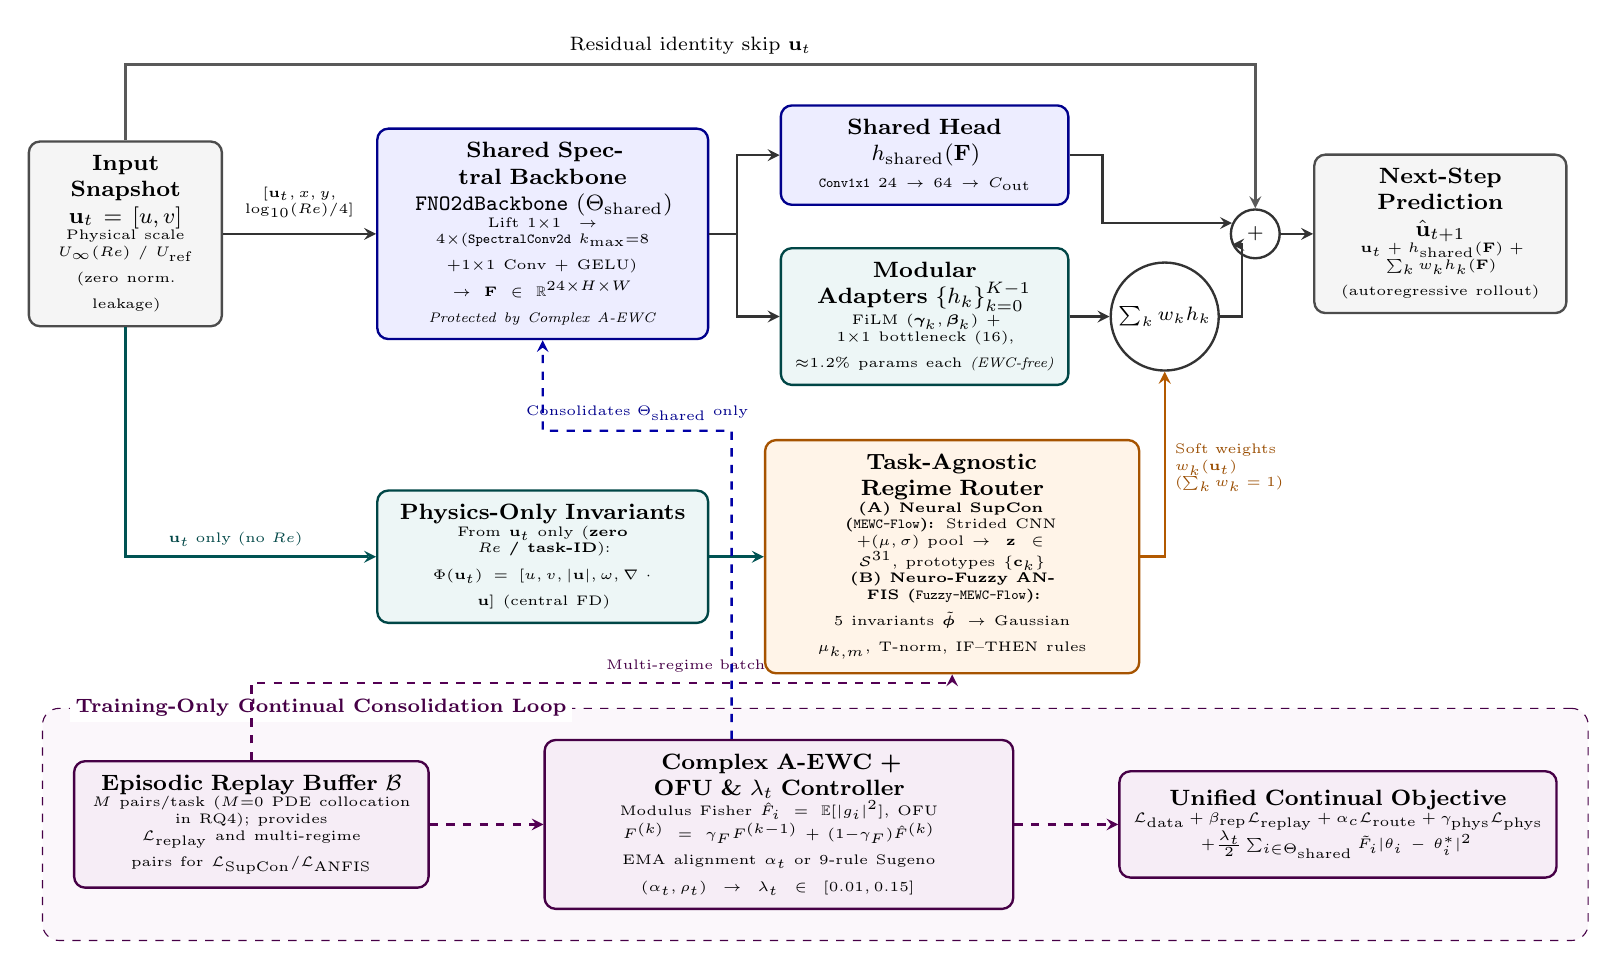
\begin{tikzpicture}[
    >=stealth,
    line width=0.85pt,
    font=\footnotesize,
    box/.style={draw=black!75, rounded corners=4pt, align=center, inner sep=5pt, minimum height=1.25cm},
    bluebox/.style={box, fill=blue!7, draw=blue!55!black},
    tealbox/.style={box, fill=teal!7, draw=teal!55!black},
    amberbox/.style={box, fill=orange!9, draw=orange!65!black},
    purplebox/.style={box, fill=violet!7, draw=violet!55!black},
    graybox/.style={box, fill=gray!8, draw=black!70},
    opcirc/.style={draw=black!80, circle, fill=white, align=center, inner sep=2pt, font=\scriptsize\bfseries},
    arr/.style={->, draw=black!80, line width=0.9pt},
    darr/.style={->, dashed, draw=black!75, line width=0.85pt}
  ]

  % --- Top Band: Shared Spectral Backbone + Modular Adapters ---
  \node[graybox, text width=2.1cm] (inp) at (0.85, 5.75) {%
    \textbf{Input Snapshot}\\
    $\mathbf{u}_t = [u, v]$\\
    {\tiny Physical scale $U_\infty(Re)$ / $U_{\text{ref}}$\\(zero norm.\ leakage)}%
  };

  \node[bluebox, text width=3.85cm] (fno) at (6.15, 5.75) {%
    \textbf{Shared Spectral Backbone}\\
    \texttt{FNO2dBackbone} ($\Theta_{\text{shared}}$)\\
    {\tiny Lift $1{\times}1 \to 4{\times}$(\texttt{SpectralConv2d} $k_{\max}{=}8$\\
    $+ 1{\times}1$ Conv + GELU) $\to \mathbf{F}\in\mathbb{R}^{24{\times}H{\times}W}$}\\
    {\tiny\itshape Protected by Complex A-EWC}%
  };

  \node[bluebox, text width=3.3cm, minimum height=1.05cm] (hshared) at (11.00, 6.75) {%
    \textbf{Shared Head} $h_{\text{shared}}(\mathbf{F})$\\
    {\tiny \texttt{Conv1x1} $24 \to 64 \to C_{\text{out}}$}%
  };

  \node[tealbox, text width=3.3cm, minimum height=1.15cm] (adapters) at (11.00, 4.70) {%
    \textbf{Modular Adapters} $\{h_k\}_{k=0}^{K-1}$\\
    {\tiny FiLM $(\boldsymbol{\gamma}_k,\boldsymbol{\beta}_k)$ + $1{\times}1$ bottleneck ($16$),\\
    ${\approx}1.2\%$ params each \textit{(EWC-free)}}%
  };

  \node[opcirc, minimum size=0.85cm] (mix) at (14.05, 4.70) {$\sum_k w_k h_k$};
  \node[opcirc, minimum size=0.62cm] (sumout) at (15.20, 5.75) {$+$};

  \node[graybox, text width=2.85cm] (out) at (17.55, 5.75) {%
    \textbf{Next-Step Prediction}\\
    $\hat{\mathbf{u}}_{t+1}$\\
    {\tiny $\mathbf{u}_t + h_{\text{shared}}(\mathbf{F}) + \sum_k w_k h_k(\mathbf{F})$\\
    (autoregressive rollout)}%
  };

  % Arrows in Top Band
  \draw[arr] (inp.east) -- node[above, align=center, font=\tiny, yshift=2pt] {$[\mathbf{u}_t, x, y,$\\$\log_{10}(Re)/4]$} (fno.west);
  \draw[arr] (fno.east) -- ++(0.35, 0) |- (hshared.west);
  \draw[arr] (fno.east) -- ++(0.35, 0) |- (adapters.west);
  \draw[arr] (adapters.east) -- (mix.west);
  \draw[arr] (hshared.east) -- ++(0.42, 0) |- (sumout.155);
  \draw[arr] (mix.east) -- ++(0.28, 0) |- (sumout.205);
  \draw[arr] (sumout.east) -- (out.west);

  % Residual skip connection
  \draw[arr, draw=black!65] (inp.north) -- (0.85, 7.90) -- node[above, font=\scriptsize] {Residual identity skip $\mathbf{u}_t$} (15.20, 7.90) -- (sumout.north);

  % --- Middle Band: Zero-Leakage Physics-Only Regime Routing ---
  \node[tealbox, text width=3.85cm, minimum height=1.2cm] (inv) at (6.15, 1.65) {%
    \textbf{Physics-Only Invariants}\\
    {\tiny From $\mathbf{u}_t$ only (\textbf{zero $Re$ / task-ID}):\\
    $\Phi(\mathbf{u}_t)=[u, v, |\mathbf{u}|, \omega, \nabla\cdot\mathbf{u}]$ (central FD)}%
  };

  \node[amberbox, text width=4.4cm, minimum height=1.45cm] (router) at (11.35, 1.65) {%
    \textbf{Task-Agnostic Regime Router}\\
    {\tiny \textbf{(A) Neural SupCon (\texttt{MEWC-Flow}):} Strided CNN\\
    $+ (\mu,\sigma)$ pool $\to \mathbf{z}\in\mathcal{S}^{31}$, prototypes $\{\mathbf{c}_k\}$\\
    \textbf{(B) Neuro-Fuzzy ANFIS (\texttt{Fuzzy-MEWC-Flow}):}\\
    5 invariants $\tilde{\boldsymbol{\phi}} \to$ Gaussian $\mu_{k,m}$, T-norm, IF--THEN rules}%
  };

  % Arrows in Middle Band
  \draw[arr, draw=teal!65!black] (inp.south) |- node[above, pos=0.72, font=\tiny, text=teal!55!black] {$\mathbf{u}_t$ only (no $Re$)} (inv.west);
  \draw[arr, draw=teal!65!black] (inv.east) -- (router.west);
  \draw[arr, draw=orange!70!black] (router.east) -| node[right, pos=0.74, align=left, font=\tiny, text=orange!60!black] {Soft weights\\$w_k(\mathbf{u}_t)$\\($\sum_k w_k=1$)} (mix.south);

  % --- Bottom Band: Training-Only Continual Consolidation Loop ---
  \node[purplebox, text width=4.15cm, minimum height=1.35cm] (replay) at (2.45, -1.75) {%
    \textbf{Episodic Replay Buffer} $\mathcal{B}$\\
    {\tiny $M$ pairs/task ($M{=}0$ PDE collocation\\
    in RQ4); provides $\mathcal{L}_{\text{replay}}$ and multi-regime\\
    pairs for $\mathcal{L}_{\text{SupCon}} / \mathcal{L}_{\text{ANFIS}}$}%
  };

  \node[purplebox, text width=5.6cm, minimum height=1.35cm] (aewc) at (9.15, -1.75) {%
    \textbf{Complex A-EWC + OFU \& $\lambda_t$ Controller}\\
    {\tiny Modulus Fisher $\hat{F}_i=\mathbb{E}[|g_i|^2]$, OFU $F^{(k)}=\gamma_F F^{(k-1)}+(1{-}\gamma_F)\hat{F}^{(k)}$\\
    EMA alignment $\alpha_t$ or 9-rule Sugeno $(\alpha_t,\rho_t)\to \lambda_t\in[0.01,0.15]$}%
  };

  \node[purplebox, text width=5.2cm, minimum height=1.35cm] (loss) at (16.25, -1.75) {%
    \textbf{Unified Continual Objective}\\
    {\tiny $\mathcal{L}_{\text{data}} + \beta_{\text{rep}}\mathcal{L}_{\text{replay}} + \alpha_c\mathcal{L}_{\text{route}} + \gamma_{\text{phys}}\mathcal{L}_{\text{phys}}$\\
    $+ \frac{\lambda_t}{2}\sum_{i\in\Theta_{\text{shared}}}\tilde{F}_i|\theta_i - \theta_i^*|^2$}%
  };

  \begin{scope}[on background layer]
    \node[draw=violet!55!black, dashed, rounded corners=6pt, fill=violet!3, fit=(replay) (aewc) (loss), inner sep=11pt, label={[font=\scriptsize\bfseries, text=violet!55!black, fill=white, inner sep=2pt, anchor=west, xshift=10pt]north west:{Training-Only Continual Consolidation Loop}}] (trainbox) {};
  \end{scope}

  % Arrows in Bottom Band (routed through open channels with zero crossings)
  \draw[darr, draw=violet!65!black] (replay.east) -- (aewc.west);
  \draw[darr, draw=violet!65!black] (aewc.east) -- (loss.west);
  \draw[darr, draw=violet!65!black] (replay.north) -- (2.45, 0.05) -- node[above, pos=0.62, font=\tiny, text=violet!55!black] {Multi-regime batch} (11.35, 0.05) -- (router.south);
  \draw[darr, draw=blue!65!black] ($(aewc.north)-(0.60,0)$) -- (8.55, 3.25) -- node[above, font=\tiny, text=blue!55!black] {Consolidates $\Theta_{\text{shared}}$ only} (6.15, 3.25) -- (fno.south);
\end{tikzpicture}%
}
\caption{End-to-end architecture of \textbf{MEWC-Flow} and neuro-fuzzy \textbf{Fuzzy-MEWC-Flow}. The shared spectral backbone (\texttt{FNO2dBackbone}, protected by complex-parameter A-EWC/OFU) extracts spatial features $\mathbf{F}$ and predicts base dynamics $h_{\text{shared}}(\mathbf{F})$, while lightweight FiLM + bottleneck adapters $\{h_k\}$ stay unconsolidated to learn regime-specific residual scales. At inference time, the router computes soft weights $w_k(\mathbf{u}_t)$ strictly from velocity invariants $\Phi(\mathbf{u}_t)$ (zero $Re$ or task-ID input), either via Supervised Contrastive prototypes (\texttt{MEWC-Flow}) or interpretable Gaussian ANFIS memberships and 9-rule Sugeno $\lambda_t$ control (\texttt{Fuzzy-MEWC-Flow}).}
\label{fig:architecture}
\end{figure}

\begin{enumerate}
  \item \textbf{Shared Spectral Backbone (\texttt{mewc\_flow/models/fno2d.py}, \texttt{surrogate.py}):}
  \begin{itemize}
    \item \emph{2D Backbone (\texttt{FNO2dBackbone}):} Concatenates $[\mathbf{u}_t, x, y, \log_{10}(Re)/4]$, lifts to width $d_h = 24$, and applies $L=4$ residual blocks pairing complex \texttt{SpectralConv2d} ($k_{\max}=8$ modes) with $1\times 1$ local convolutions and GELU ($299{,}186$ base params; $340{,}018$ modular params).
    \item \emph{1D Backbone (\texttt{FNO1d}):} Uses $L=3$ blocks with $d_h=32$, $k_{\max}=16$ modes ($54{,}625$ base / $76{,}065$ modular params). Both predict residual increments $\hat{\mathbf{u}}_{t+1} = \mathbf{u}_t + \Delta\hat{\mathbf{u}}$.
  \end{itemize}

  \item \textbf{Physics-Only Supervised Contrastive Regime Encoder (RQ3):} Operates \emph{strictly} on flow-derived spatial invariants computed via central finite differences from velocity alone (\textbf{zero $Re$ or task-ID input}):
  \begin{equation}
  \Phi(\mathbf{u}_t) = \left[u, \; v, \; \sqrt{u^2 + v^2 + \epsilon}, \; \omega = \frac{\partial v}{\partial x} - \frac{\partial u}{\partial y}, \; \delta = \frac{\partial u}{\partial x} + \frac{\partial v}{\partial y}\right] \in \mathbb{R}^{5 \times H \times W},
  \end{equation}
  (and $\Phi_{1\text{d}}(u_t) = [u, u_x, u_{xx}]$ in 1D). A strided CNN pools spatial means and standard deviations into $\mathbf{z}(\mathbf{u}_t) \in \mathcal{S}^{31}$ trained with Supervised Contrastive Loss~\cite{khosla2020supcon} ($\tau_c = 0.10$, $\alpha_c = 0.25$) over replay-augmented batches. Normalized prototypes $\mathbf{c}_k$ freeze after each stage, enabling task-agnostic soft routing at test time:
  \begin{equation}
  w_k(\mathbf{u}_t) = \frac{\exp(\mathbf{z}(\mathbf{u}_t)^{\top} \mathbf{c}_k / \tau_{\text{route}})}{\sum_{m=0}^{K-1} \exp(\mathbf{z}(\mathbf{u}_t)^{\top} \mathbf{c}_m / \tau_{\text{route}})}, \qquad \hat{\mathbf{u}}_{t+1} = \mathbf{u}_t + h_{\text{shared}}(\mathbf{F}) + \sum_{k=0}^{K-1} w_k(\mathbf{u}_t)\, h_k(\mathbf{F}).
  \end{equation}

  \item \textbf{Lightweight Modular Regime Adapters:} Each regime adapter $h_k$ applies FiLM modulation $(\boldsymbol{\gamma}_k, \boldsymbol{\beta}_k)$ and a $1\times 1$ bottleneck residual head (width 16, $\approx 1.2\%$ of backbone parameters), excluded from EWC stiffness so each regime adapts amplitude scales freely.

  \item \textbf{Complex-Parameter Adaptive EWC (A-EWC) \& Online Fisher Updating (\texttt{ewc.py}):} Extends MEWC-RL++~\cite{hasan2026mewcrlpp} to complex weights $\theta_i \in \mathbb{C}$ via strictly real modulus-squared Fisher $\hat{F}_i^{(k)} = \mathbb{E}[|\partial \ell / \partial \theta_i|^2]$, exact sample normalization, empirical-Bayes scaling (\texttt{task\_mse}, natural radius $r_0^2 = 10^{-6}$), and $\mathcal{O}(|\Theta_{\text{shared}}|)$ Online Fisher Updating ($F^{(k)} = \gamma_F F^{(k-1)} + (1-\gamma_F)\hat{F}^{(k)}$, $\gamma_F = 0.85$) restricted to a shared-backbone parameter allowlist. EMA gradient cosine alignment $\alpha_t \in [-1, 1]$ ($\beta_g = 0.9$) modulates $\lambda_t = \lambda_{\min} + \left(1 - \frac{1+\alpha_t}{2}\right)(\lambda_{\max} - \lambda_{\min}) \in [0.01, 0.15]$, increasing consolidation during gradient conflicts ($\alpha_t < 0$).

  \item \textbf{Combined Objective, Matched Replay \& Fair Optimization:} Minimizes $\mathcal{L}_{\text{data}}^{(k)} + \beta_{\text{rep}}\mathcal{L}_{\text{replay}} + \alpha_c \mathcal{L}_{\text{SupCon}} + \gamma_{\text{phys}}\mathcal{L}_{\text{phys}} + \frac{\lambda_t}{2}\sum_{i\in\Theta_{\text{shared}}} \tilde{F}_i|\theta_i - \theta_i^*|^2$ ($\beta_{\text{rep}}=1.0$, $\gamma_{\text{phys}}=0.05$ 2D vorticity/divergence or $0.02$ 1D Burgers PDE). For \texttt{MEWC-PDE-Replay} (RQ4), episodic storage is $M=0$ (\texttt{use\_replay=False}) with differentiable PDE-residual supervision on collocation points. All methods use identical \texttt{Adam} ($\text{lr}=10^{-3}$), \texttt{CosineAnnealingLR} ($\eta_{\min}=0.01\cdot\text{lr}$), and gradient norm clipping at $1.0$ (Algorithm~\ref{alg:mewcflow}).

  \item \textbf{Neuro-Fuzzy Extension (\texttt{Fuzzy-MEWC-Flow}, \texttt{fuzzy\_logic.py}):} Replaces black-box routing and linear $\lambda_t$ scaling with two principled fuzzy components~\cite{mamdani1974fuzzy,takagi1985fuzzy,jang1993anfis}: (a) \texttt{TakagiSugenoRegimeRouter} learning Gaussian memberships $\mu_{k,m}(\tilde{\phi}_m)$ ($\sigma_{k,m} \ge 0.20$) over 5 dimensionless 2D invariants ($[\text{KE}, \text{TKE}_{\text{var}}, \log(1+\text{Enstrophy}), \log(1+\sigma_{\omega}), \log(1+\|\nabla\cdot\mathbf{u}\|^2)]$; standardized strictly on Task-0 with zero $Re$ input) combined via log-space product T-norm and softmax ($\tau_{\text{fuzzy}}=1.0$) to export linguistic IF--THEN rules; and (b) \texttt{FuzzyAdaptiveEWC}, a 9-rule zero-order Sugeno controller mapping $(\alpha_t, \rho_t) \in [-1,1]^2$ into $\lambda_t \in [0.01, 0.15]$.
\end{enumerate}

\begin{algorithm}[!htbp]
\caption{MEWC-Flow Continual Learning \& Task-Agnostic Inference}
\label{alg:mewcflow}
\begin{algorithmic}[1]
\REQUIRE Sequential tasks $\{\mathcal{D}_k^{\text{train}}\}_{k=0}^{K-1}$, shared FNO backbone $\Theta_{\text{shared}}$, adapters $\{h_k\}_{k=0}^{K-1}$, physics-only encoder $e_{\psi}$, episodic buffer $\mathcal{B}$ (cap $M$/task), bounds $[\lambda_{\min}, \lambda_{\max}]$.
\STATE Initialize $\mathbf{g}_{\text{prev}} \gets \mathbf{0}$, $\mathcal{B} \gets \emptyset$.
\FOR{$k = 0, \dots, K-1$}
  \STATE Train with \texttt{Adam} ($\text{lr}=10^{-3}$) + \texttt{CosineAnnealingLR} over active parameters:
  \FOR{each mini-batch $(\mathbf{u}_t, \mathbf{u}_{t+1}) \sim \mathcal{D}_k^{\text{train}}$}
    \STATE Compute $\mathcal{L}_{\text{data}}^{(k)}$ + $\mathcal{L}_{\text{phys}}$; if $k>0$ and $|\mathcal{B}|>0$, sample replay $(\mathbf{u}_r, \mathbf{u}_{r+1}, y_r)\sim\mathcal{B}$ to compute $\mathcal{L}_{\text{replay}}$, $\mathcal{L}_{\text{SupCon}}$ on $\Phi(\mathbf{u})$, alignment $\alpha_t \to \lambda_t$, and Complex A-EWC penalty on $\Theta_{\text{shared}}$.
    \STATE Step optimizer with $\|\mathbf{g}\|_2 \le 1.0$ clipping and update EMA gradient memory $\mathbf{g}_{\text{prev}}$.
  \ENDFOR
  \STATE Freeze prototype $\mathbf{c}_k \gets \text{norm}(\mathbb{E}_{\mathcal{D}_k}[e_{\psi}(\Phi(\mathbf{u}))])$; store $M$ exemplars in $\mathcal{B}$; update OFU Fisher $F^{(k)} \gets \gamma_F F^{(k-1)} + (1-\gamma_F)\hat{F}^{(k)}$.
\ENDFOR
\STATE \textbf{Task-Agnostic Inference:} Extract $\mathbf{z}=e_{\psi}(\Phi(\mathbf{u}_t))$ (zero $Re$ input), compute soft weights $w_k$, and output $\hat{\mathbf{u}}_{t+1} = \mathbf{u}_t + h_{\text{shared}}(\mathbf{F}) + \sum_k w_k h_k(\mathbf{F})$.
\end{algorithmic}
\end{algorithm}

\FloatBarrier
% ==============================================================================
\section{Experimental Suite \& Verified Findings}
% ==============================================================================

We evaluate MEWC-Flow against seven matched baselines (\texttt{Fine-Tuning}, \texttt{EWC}, \texttt{Online-EWC}, \texttt{ER}~\cite{rolnick2019er}, \texttt{Replay-TS}~\cite{hemati2026replayts}, \texttt{SLE-FNO}~\cite{elhadidy2026slefno}, offline \texttt{Joint}, plus \texttt{MEWC-PDE-Replay} on Burgers) across four benchmarks with exact byte-level memory accounting (\texttt{Extra MB}).

\subsection{Benchmark 1: Experimental Caltech PIV Cylinder Wakes (5 Seeds, $M=16$)}

Real planar velocity $(u, v)$ on $64\times 64$ grids across $Re = 240 \to 650 \to 1280 \to 2520$ (held-out $Re = 910, 1890$; 15 epochs/task; seeds \texttt{42, 102, 202, 302, 402})~\cite{renn2026piv}. \texttt{Fine-Tuning} degrades Task-0 by $+134.8\%$ ($\text{VPH}_{0.25}=14.3\pm 5.6$ steps vs.\ $20.0\pm 0.0$ for MEWC-Flow). \texttt{MEWC-Flow} matches \texttt{Joint} Final MSE ($1.05\times 10^{-3}$, $p=0.731$) and beats \texttt{EWC}, \texttt{Online-EWC}, \texttt{Replay-TS}, and \texttt{SLE-FNO} ($p \le 0.002$), while achieving the lowest seed-0 inertial-band spectral error ($0.0484$ vs.\ \texttt{ER} $0.0794$, \texttt{Fine-Tuning} $0.3287$). Monolithic \texttt{ER} obtains marginally lower single-step MSE ($1.03\times 10^{-3}$, $p=0.015$) with lower RAM ($4.20\text{ MB}$) and ties on rollout ($0.0997$, $p=0.996$; Tables~\ref{tab:piv_main}--\ref{tab:piv_stats}, Figs.~\ref{fig:piv_main}--\ref{fig:piv_physics}).

\begin{table}[!htbp]
\centering
\caption{Caltech PIV cylinder wake benchmark ($5$ seeds, $15$ epochs/task, $M=16$). Significance compares each baseline vs.\ MEWC-Flow ($^{*}p<0.05$, $^{**}p<0.01$, paired two-sided $t$-test).}
\label{tab:piv_main}
\resizebox{\textwidth}{!}{%
\begin{tabular}{@{}lcccccc@{}}
\toprule
Method & Avg.\ Forgetting ($\Delta$MSE) & Final MSE (4 regimes) & $Re=240$ Rollout Rel-$L_2$ ($t=10$) & $Re=240$ Vorticity RMSE & Held-out MSE ($Re=910, 1890$) & Extra Memory (MB) \\
\midrule
Fine-Tuning & $4.34 \times 10^{-4} \pm 4.1 \times 10^{-4}$$^{*}$ & $1.43 \times 10^{-3} \pm 3.1 \times 10^{-4}$$^{*}$ & $0.2125 \pm 0.0633$$^{*}$ & $0.0358 \pm 0.0057$ & $1.51 \times 10^{-3} \pm 1.9 \times 10^{-4}$$^{*}$ & 0.00 \\
EWC & $-2.25 \times 10^{-5} \pm 5.0 \times 10^{-6}$$^{**}$ & $1.26 \times 10^{-3} \pm 9.1 \times 10^{-6}$$^{**}$ & $0.1059 \pm 0.0053$ & $0.0280 \pm 0.0007$ & $1.50 \times 10^{-3} \pm 1.3 \times 10^{-5}$$^{**}$ & 3.57 \\
Online-EWC & $-1.09 \times 10^{-5} \pm 2.6 \times 10^{-5}$$^{**}$ & $1.24 \times 10^{-3} \pm 1.8 \times 10^{-5}$$^{**}$ & $0.1230 \pm 0.0237$ & $0.0289 \pm 0.0015$ & $1.47 \times 10^{-3} \pm 1.7 \times 10^{-5}$$^{**}$ & 3.57 \\
ER & $-8.02 \times 10^{-5} \pm 9.6 \times 10^{-6}$ & $1.03 \times 10^{-3} \pm 1.2 \times 10^{-5}$$^{*}$ & $0.0997 \pm 0.0043$ & $0.0279 \pm 0.0017$ & $1.26 \times 10^{-3} \pm 1.0 \times 10^{-5}$$^{*}$ & 4.20 \\
Replay-TS & $-7.94 \times 10^{-5} \pm 9.7 \times 10^{-6}$ & $1.06 \times 10^{-3} \pm 1.6 \times 10^{-5}$$^{**}$ & $0.0981 \pm 0.0019$ & $0.0270 \pm 0.0012$ & $1.29 \times 10^{-3} \pm 1.9 \times 10^{-5}$ & 3.93 \\
SLE-FNO & $2.60 \times 10^{-7} \pm 2.8 \times 10^{-7}$$^{**}$ & $1.34 \times 10^{-3} \pm 6.0 \times 10^{-6}$$^{**}$ & $0.1237 \pm 0.0029$$^{**}$ & $0.0320 \pm 0.0006$$^{*}$ & $1.59 \times 10^{-3} \pm 5.7 \times 10^{-6}$$^{**}$ & 0.01 \\
\textbf{MEWC-Flow} & $\mathbf{-7.78 \times 10^{-5} \pm 1.8 \times 10^{-5}}$ & $\mathbf{1.05 \times 10^{-3} \pm 1.7 \times 10^{-5}}$ & $\mathbf{0.0997 \pm 0.0053}$ & $\mathbf{0.0278 \pm 0.0020}$ & $\mathbf{1.28 \times 10^{-3} \pm 2.1 \times 10^{-5}}$ & \textbf{10.32} \\
Joint & $0.00 \times 10^{0} \pm 0.0 \times 10^{0}$$^{**}$ & $1.05 \times 10^{-3} \pm 4.3 \times 10^{-5}$ & $0.0853 \pm 0.0043$$^{**}$ & $0.0242 \pm 0.0015$$^{*}$ & $1.28 \times 10^{-3} \pm 5.0 \times 10^{-5}$ & 38.80 \\
\bottomrule
\end{tabular}%
}
\end{table}

\begin{table}[!htbp]
\centering
\caption{Paired two-sided $t$-tests and Cohen's $d$ on Caltech PIV (MEWC-Flow minus baseline across 5 seeds). Negative $\Delta$ and $d < 0$ favor MEWC-Flow.}
\label{tab:piv_stats}
\resizebox{\textwidth}{!}{%
\begin{tabular}{@{}lccccc@{}}
\toprule
Comparison & $\Delta$Final MSE ($p$) & $\Delta$Forgetting ($p$) & $\Delta$Rollout $t=10$ ($p$) & $\Delta$Held-out MSE ($p$) & Cohen's $d$ (Final MSE) \\
\midrule
MEWC-Flow vs.\ Fine-Tuning & $-3.80 \times 10^{-4}$ (0.047) & $-5.12 \times 10^{-4}$ (0.045) & $-0.1127$ (0.020) & $-2.26 \times 10^{-4}$ (0.043) & $-1.27$ \\
MEWC-Flow vs.\ EWC & $-2.11 \times 10^{-4}$ (0.000) & $-5.52 \times 10^{-5}$ (0.001) & $-0.0061$ (0.228) & $-2.20 \times 10^{-4}$ (0.000) & $-13.97$ \\
MEWC-Flow vs.\ Online-EWC & $-1.93 \times 10^{-4}$ (0.000) & $-6.69 \times 10^{-5}$ (0.002) & $-0.0233$ (0.135) & $-1.89 \times 10^{-4}$ (0.000) & $-12.38$ \\
MEWC-Flow vs.\ ER & $+1.34 \times 10^{-5}$ (0.015) & $+2.41 \times 10^{-6}$ (0.745) & $-0.0000$ (0.996) & $+2.12 \times 10^{-5}$ (0.033) & $+1.84$ \\
MEWC-Flow vs.\ Replay-TS & $-1.49 \times 10^{-5}$ (0.002) & $+1.60 \times 10^{-6}$ (0.811) & $+0.0016$ (0.400) & $-6.56 \times 10^{-6}$ (0.398) & $-3.02$ \\
MEWC-Flow vs.\ SLE-FNO & $-2.94 \times 10^{-4}$ (0.000) & $-7.80 \times 10^{-5}$ (0.001) & $-0.0240$ (0.001) & $-3.13 \times 10^{-4}$ (0.000) & $-14.93$ \\
MEWC-Flow vs.\ Joint & $-5.71 \times 10^{-6}$ (0.731) & $-7.78 \times 10^{-5}$ (0.001) & $+0.0144$ (0.010) & $+2.02 \times 10^{-6}$ (0.916) & $-0.17$ \\
\bottomrule
\end{tabular}%
}
\end{table}

\begin{figure}[!htbp]
\centering
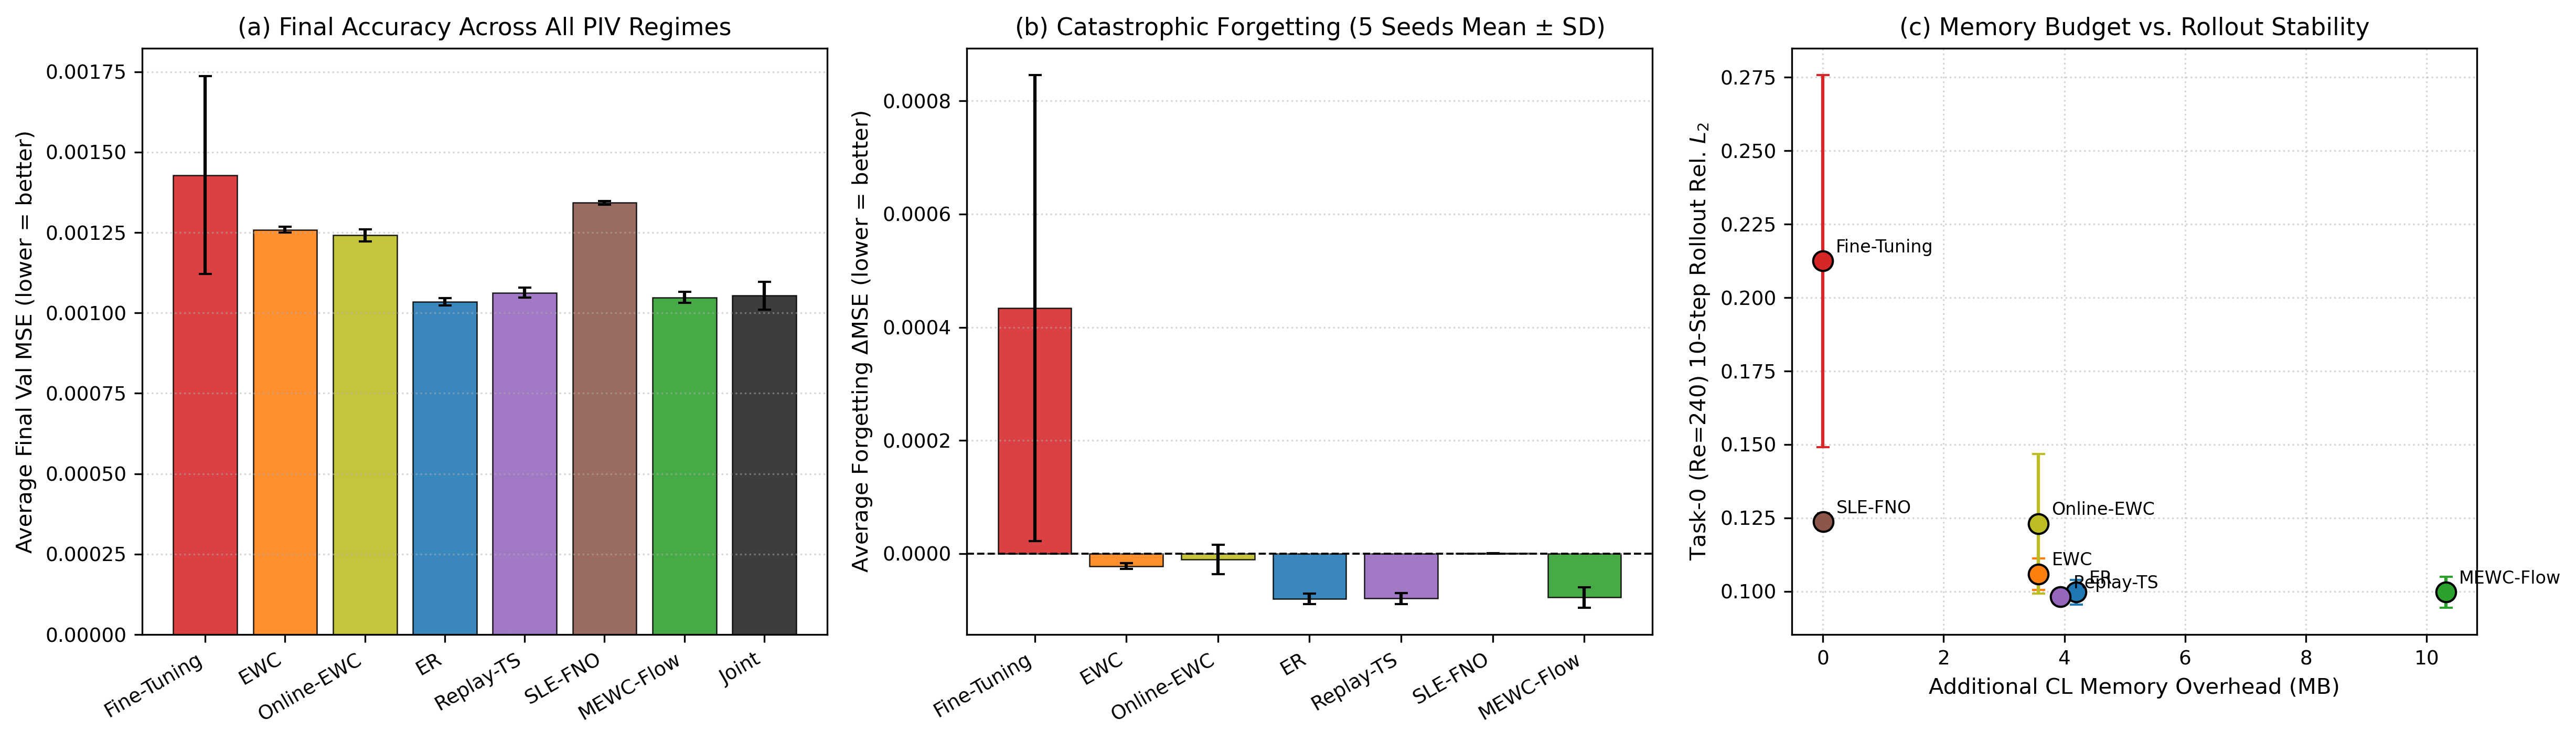
\includegraphics[width=0.96\textwidth,height=0.39\textheight,keepaspectratio]{figures/fig1_piv_benchmark_and_forgetting.png}
\caption{Caltech PIV benchmark across 5 random seeds ($M=16$, 15 epochs/task): final MSE, catastrophic forgetting ($\Delta$MSE), Task-0 degradation, and held-out cross-$Re$ generalization.}
\label{fig:piv_main}
\end{figure}

\begin{figure}[!htbp]
\centering
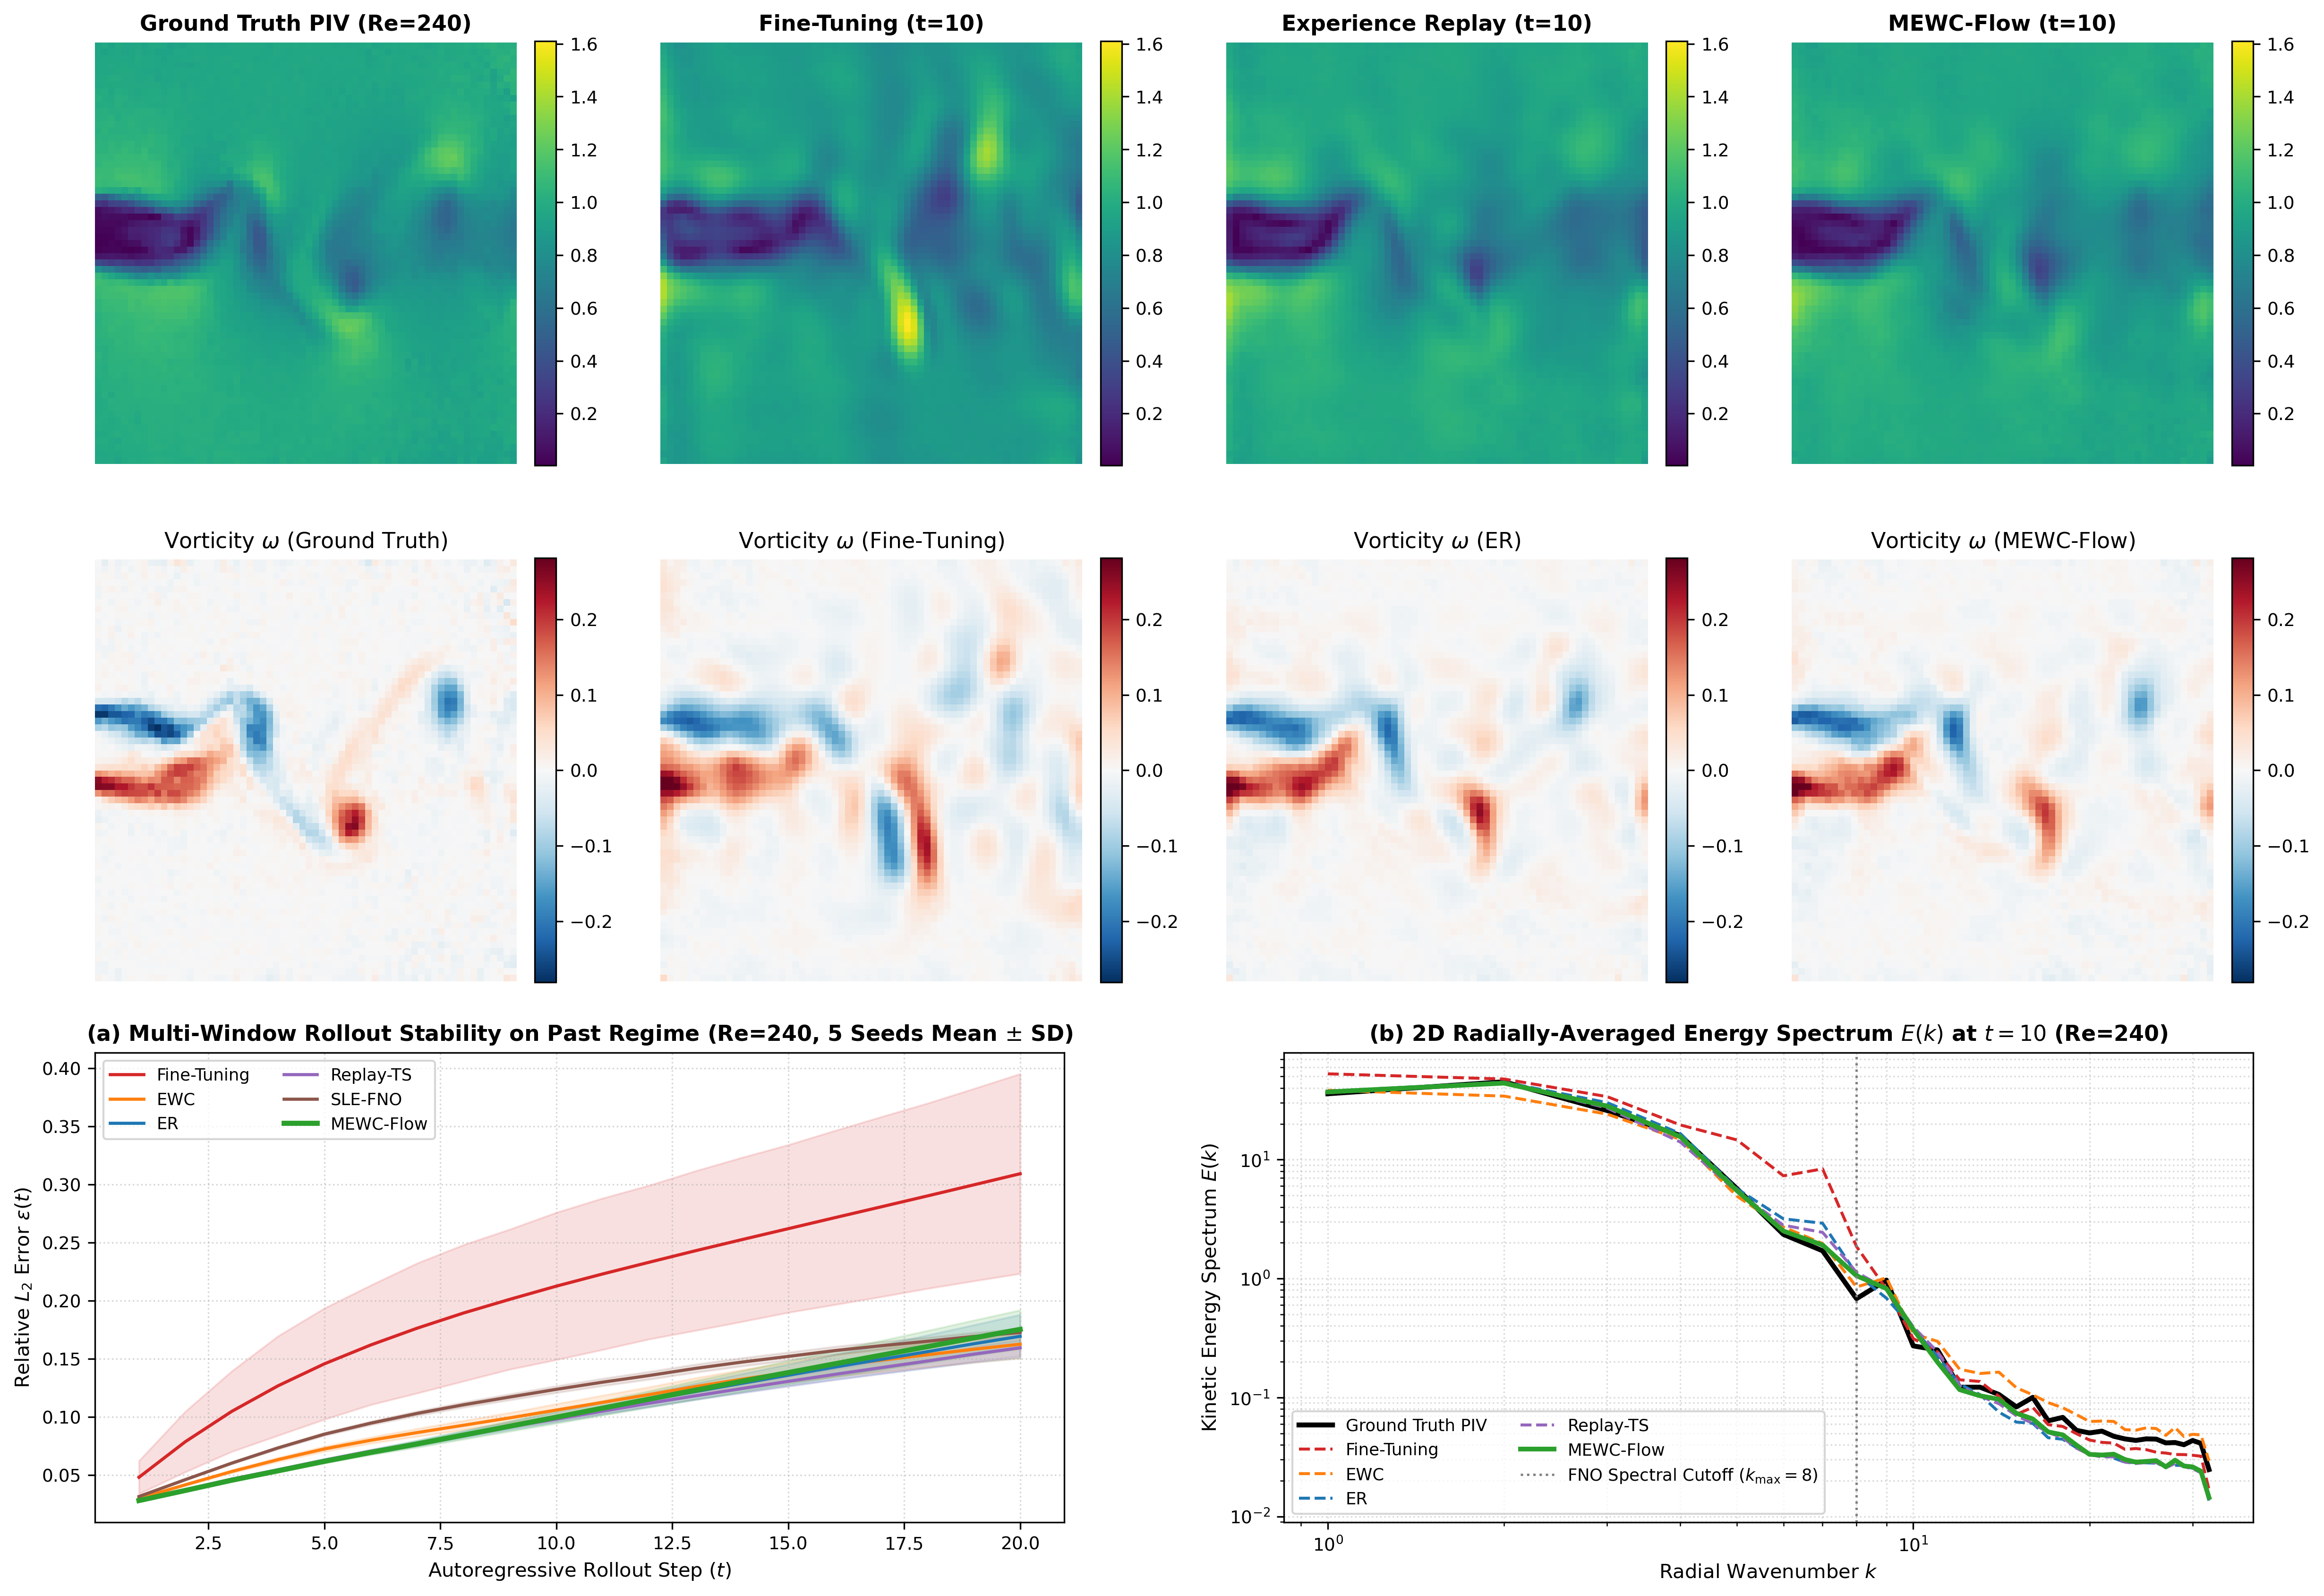
\includegraphics[width=0.96\textwidth,height=0.39\textheight,keepaspectratio]{figures/fig2_piv_physics_rollout_spectrum.png}
\caption{Physical and spectral diagnostics on $Re=240$ after learning up to $Re=2520$: vorticity snapshots, divergence RMSE, radial spectra $E(k)$, and autoregressive rollout drift.}
\label{fig:piv_physics}
\end{figure}

\FloatBarrier
\subsection{Zero-Leakage Physics-Only Regime Identification \& Routing (RQ3)}

Without any $Re$ input, \texttt{PhysicsRegimeEncoder2d} attains $\mathbf{77.55\% \pm 4.61\%}$ regime accuracy across 5 seeds (silhouette $0.4647 \pm 0.0560$) and $\mathbf{84.2\%}$ on seed-0 (silhouette $0.518$; Fig.~\ref{fig:piv_latent}), with $100\%$ separation on $Re \in \{240, 1280, 2520\}$ and all misclassifications confined to adjacent shedding overlap ($Re=650 \leftrightarrow 1280$). Held-out regimes $Re=910^*$ and $1890^*$ receive smooth interpolation weights (Table~\ref{tab:routing_weights}).

\begin{table}[!htbp]
\centering
\caption{Soft routing attention weights $w_k(\mathbf{u}_t)$ produced by the seed-0 MEWC-Flow encoder without $Re$ input ($^*$ denotes zero-shot unseen held-out Reynolds regimes).}
\label{tab:routing_weights}
\begin{tabular}{@{}lcccc@{}}
\toprule
Input Regime & Adapter $Re=240$ & Adapter $Re=650$ & Adapter $Re=1280$ & Adapter $Re=2520$ \\
\midrule
$Re=240$ & \textbf{0.97} & 0.03 & 0.00 & 0.00 \\
$Re=650$ & 0.00 & \textbf{0.64} & 0.36 & 0.00 \\
$Re=910^*$ & 0.00 & 0.07 & \textbf{0.92} & 0.00 \\
$Re=1280$ & 0.00 & 0.02 & \textbf{0.98} & 0.00 \\
$Re=1890^*$ & 0.00 & 0.00 & 0.04 & \textbf{0.96} \\
$Re=2520$ & 0.00 & 0.00 & 0.00 & \textbf{1.00} \\
\bottomrule
\end{tabular}
\end{table}

\begin{figure}[!htbp]
\centering
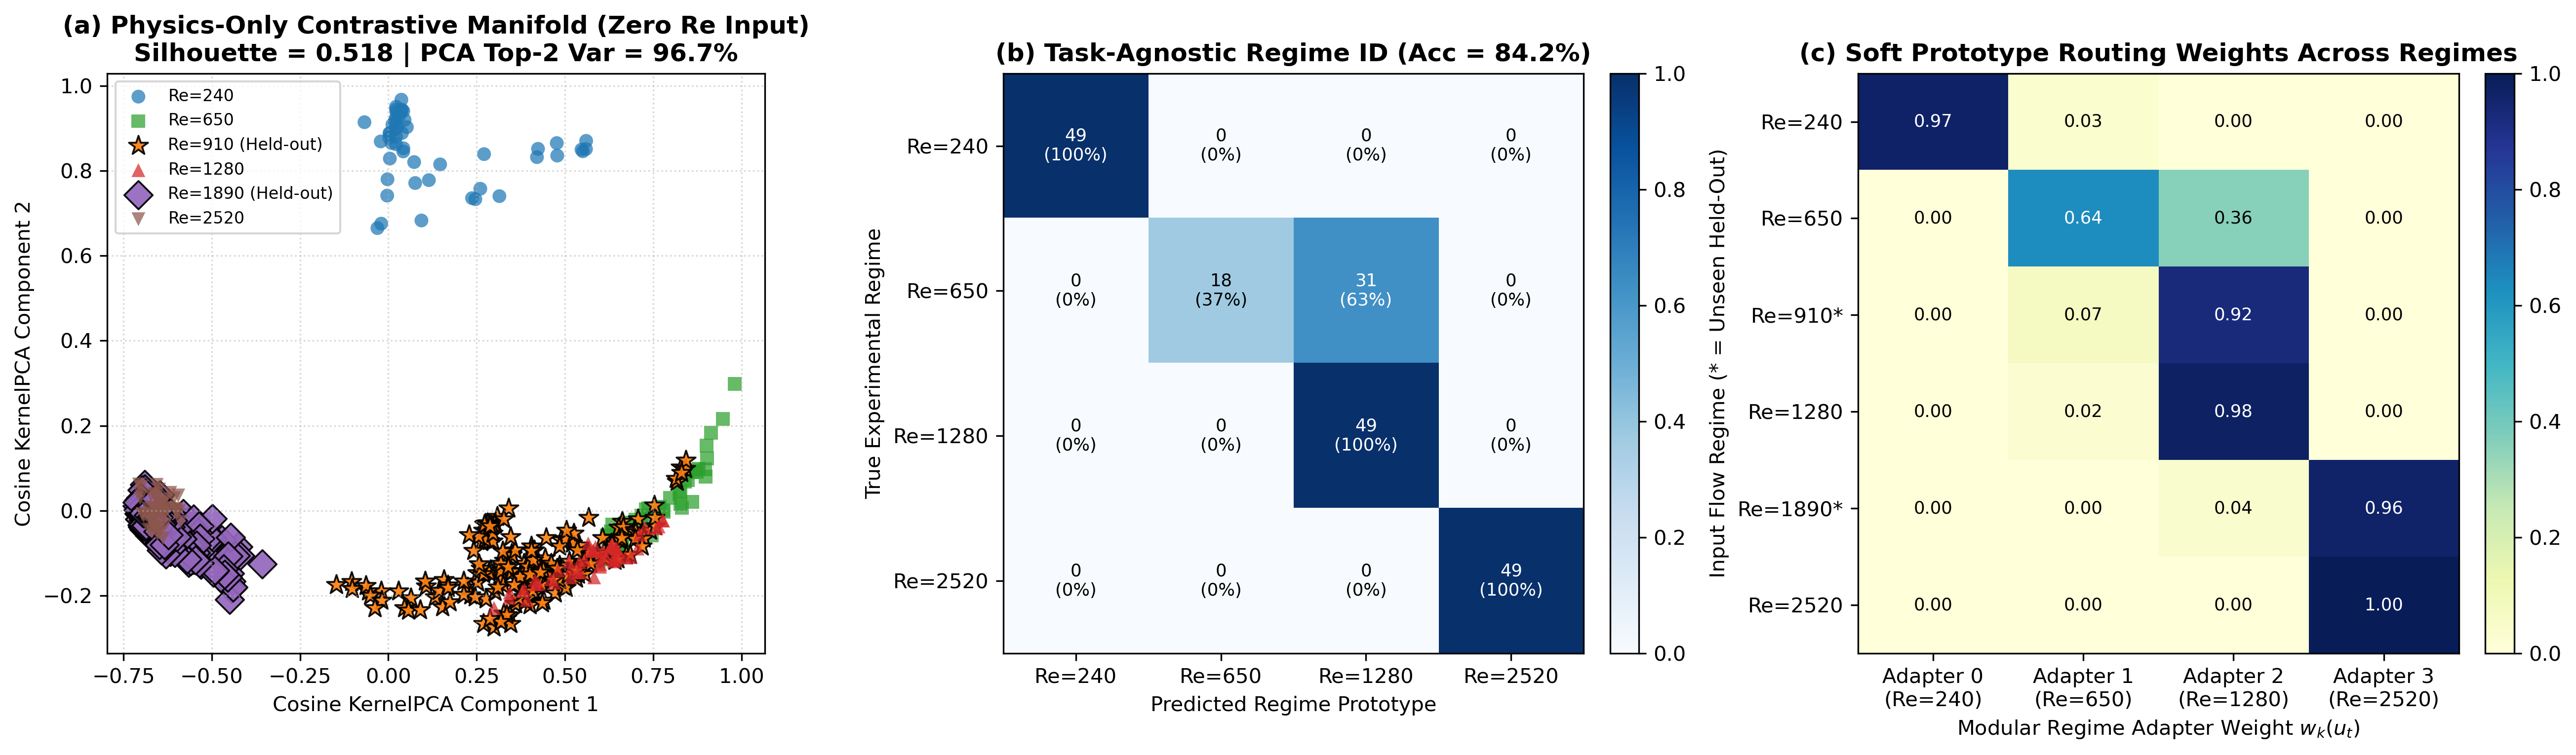
\includegraphics[width=0.96\textwidth,height=0.39\textheight,keepaspectratio]{figures/fig3_piv_latent_manifold_and_routing.png}
\caption{PCA projection of the zero-leakage contrastive latent space (left) and soft routing matrix across seen and held-out Reynolds numbers (right).}
\label{fig:piv_latent}
\end{figure}

\FloatBarrier
\subsection{Benchmark 2: 2D Kolmogorov Navier--Stokes Bifurcation ($Re=20 \to 400$, 3 Seeds)}

Pseudo-spectral RK4 incompressible 2D NS on $[0, 2\pi]^2$ ($64\times 64$) across steady ($Re=20$), bifurcation onset ($45$), transitional ($120$), and turbulent ($400$) regimes (held-out $75, 240$; 12 epochs/task; $M=16$). \texttt{MEWC-Flow} achieves the \textbf{global lowest exact 2D NS PDE residual ($7.040 \pm 0.017$)}, significantly beating \texttt{ER} ($7.386$, $p=0.0035$), \texttt{Replay-TS} ($7.365$, $p=0.0030$), \texttt{EWC} ($8.316$, $p=0.0015$), \texttt{SLE-FNO} ($9.090$, $p<10^{-4}$), and offline \texttt{Joint} ($7.120$, $p=0.0149$), while trading a small 1-step MSE margin against monolithic \texttt{ER} ($3.31\times 10^{-3}$ vs.\ $2.99\times 10^{-3}$; Table~\ref{tab:kolmogorov}, Fig.~\ref{fig:kolmogorov}).

\begin{table}[!htbp]
\centering
\caption{2D Kolmogorov Navier--Stokes bifurcation benchmark ($Re = 20 \to 45 \to 120 \to 400$, held-out $Re = 75, 240$; 3 seeds, 12 epochs/task, $M = 16$).}
\label{tab:kolmogorov}
\resizebox{\textwidth}{!}{%
\begin{tabular}{@{}lccccccc@{}}
\toprule
Method & Avg.\ Forgetting & Final MSE & NS PDE Residual (RMS) & $\|\nabla \cdot \mathbf{u}\|$ RMS & Rollout $t=10$ (mean of 4) & Held-out MSE ($Re=75, 240$) & Extra MB \\
\midrule
Fine-Tuning & $-8.29 \times 10^{-4} \pm 5.0 \times 10^{-5}$ & $3.60 \times 10^{-3} \pm 1.5 \times 10^{-4}$$^{*}$ & $7.846 \pm 0.112$$^{**}$ & $0.6490 \pm 0.0679$ & $0.4670 \pm 0.0375$$^{*}$ & $5.14 \times 10^{-3} \pm 2.2 \times 10^{-4}$$^{*}$ & 0.00 \\
EWC & $-5.81 \times 10^{-4} \pm 1.4 \times 10^{-4}$ & $6.88 \times 10^{-3} \pm 8.6 \times 10^{-4}$$^{*}$ & $8.316 \pm 0.093$$^{**}$ & $0.7846 \pm 0.1250$ & $0.5079 \pm 0.0079$$^{**}$ & $1.09 \times 10^{-2} \pm 1.5 \times 10^{-3}$$^{*}$ & 3.57 \\
Online-EWC & $-9.95 \times 10^{-4} \pm 3.3 \times 10^{-4}$ & $4.55 \times 10^{-3} \pm 3.7 \times 10^{-4}$$^{**}$ & $8.044 \pm 0.089$$^{**}$ & $0.8097 \pm 0.0954$ & $0.4743 \pm 0.0412$$^{*}$ & $6.79 \times 10^{-3} \pm 5.8 \times 10^{-4}$$^{**}$ & 3.57 \\
ER & $-1.22 \times 10^{-3} \pm 8.0 \times 10^{-5}$$^{*}$ & $2.99 \times 10^{-3} \pm 7.7 \times 10^{-5}$ & $7.386 \pm 0.045$$^{**}$ & $0.4732 \pm 0.0210$ & $0.3054 \pm 0.0020$$^{*}$ & $4.52 \times 10^{-3} \pm 1.4 \times 10^{-4}$ & 4.20 \\
Replay-TS & $-1.19 \times 10^{-3} \pm 7.5 \times 10^{-5}$$^{*}$ & $3.00 \times 10^{-3} \pm 7.7 \times 10^{-5}$ & $7.365 \pm 0.041$$^{**}$ & $0.4535 \pm 0.0085$ & $0.2966 \pm 0.0012$$^{*}$ & $4.59 \times 10^{-3} \pm 1.1 \times 10^{-4}$ & 3.93 \\
SLE-FNO & $-8.88 \times 10^{-6} \pm 4.4 \times 10^{-6}$$^{**}$ & $1.25 \times 10^{-2} \pm 1.9 \times 10^{-5}$$^{**}$ & $9.090 \pm 0.006$$^{**}$ & $0.2145 \pm 0.0451$ & $0.6905 \pm 0.0006$$^{**}$ & $2.26 \times 10^{-2} \pm 5.5 \times 10^{-5}$$^{**}$ & 0.01 \\
\textbf{MEWC-Flow} & $\mathbf{-1.00 \times 10^{-3} \pm 1.3 \times 10^{-4}}$ & $\mathbf{3.31 \times 10^{-3} \pm 1.8 \times 10^{-4}}$ & $\mathbf{7.040 \pm 0.017}$ & $\mathbf{0.5260 \pm 0.0237}$ & $\mathbf{0.3442 \pm 0.0092}$ & $\mathbf{4.80 \times 10^{-3} \pm 2.7 \times 10^{-4}}$ & \textbf{10.32} \\
Joint & $0.00 \times 10^{0} \pm 0.0 \times 10^{0}$$^{**}$ & $2.34 \times 10^{-3} \pm 4.4 \times 10^{-5}$$^{**}$ & $7.120 \pm 0.017$$^{*}$ & $0.3778 \pm 0.0240$ & $0.2307 \pm 0.0048$$^{**}$ & $3.53 \times 10^{-3} \pm 7.5 \times 10^{-5}$$^{**}$ & 46.14 \\
\bottomrule
\end{tabular}%
}
\end{table}

\begin{figure}[!htbp]
\centering
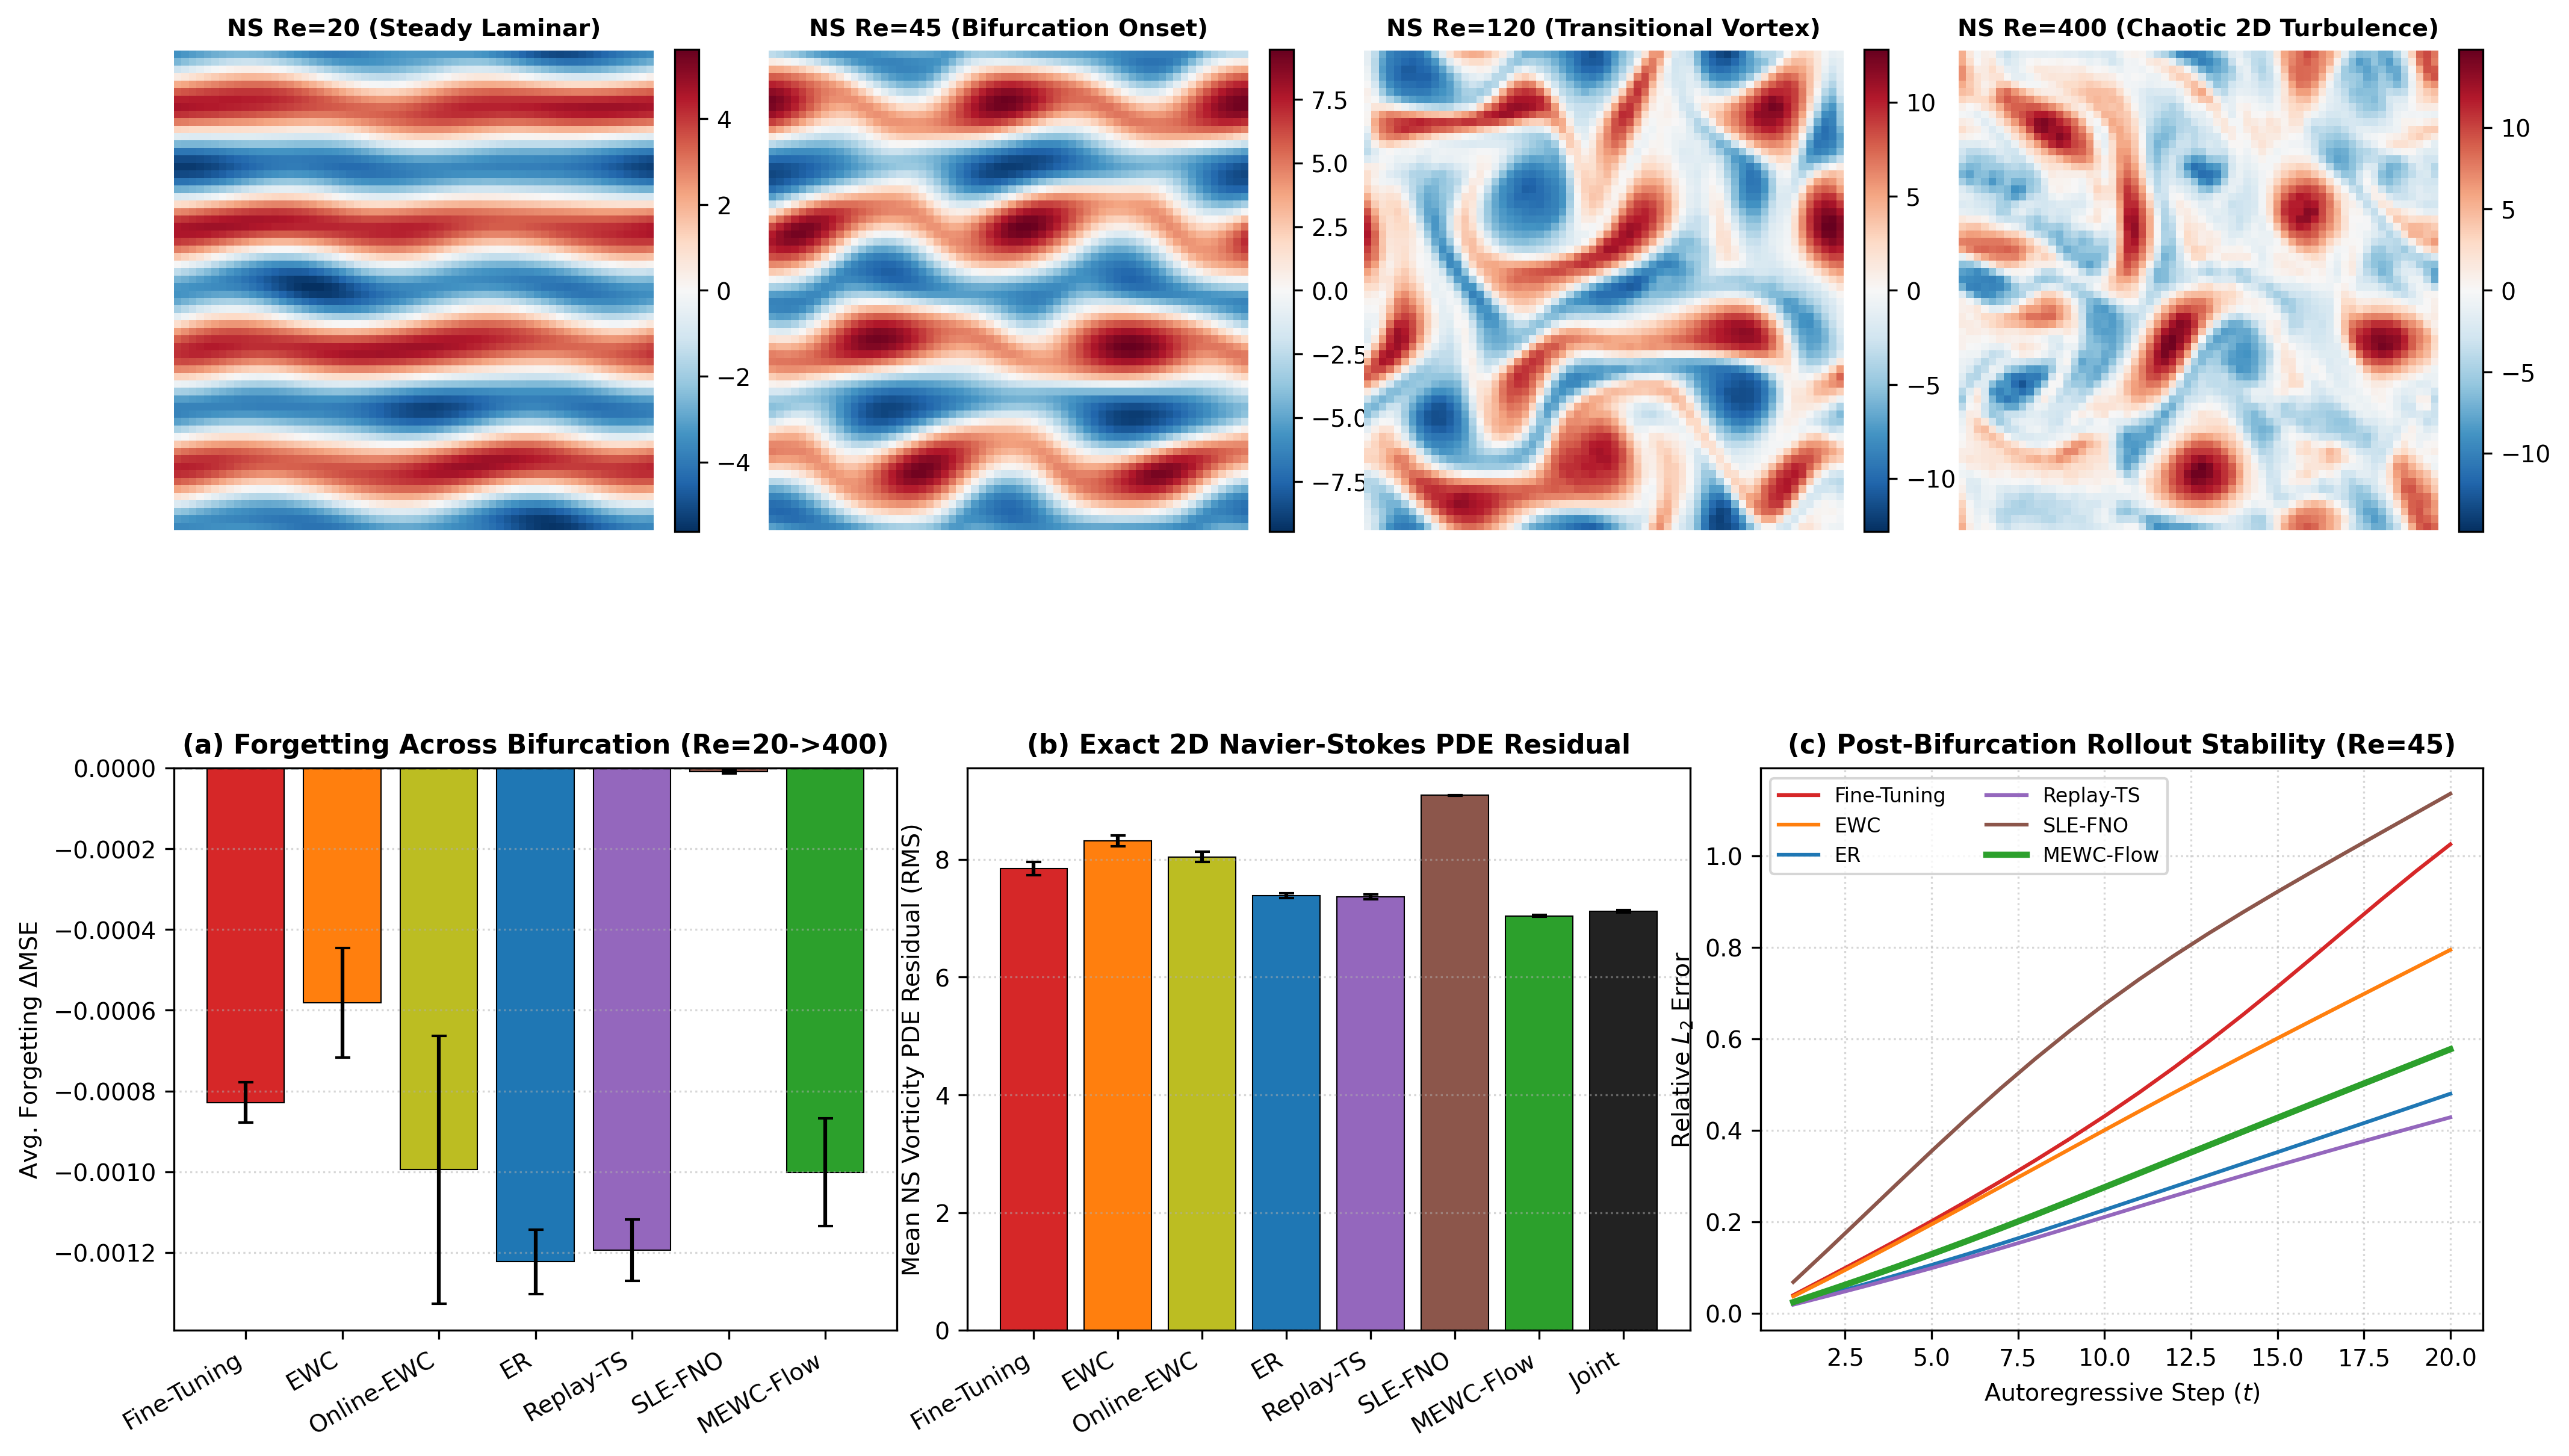
\includegraphics[width=0.96\textwidth,height=0.39\textheight,keepaspectratio]{figures/fig5_kolmogorov_bifurcation.png}
\caption{2D Kolmogorov Navier--Stokes bifurcation ($Re=20 \to 400$): vorticity snapshots, forgetting, exact NS PDE residual, and post-bifurcation $Re=45$ rollout stability.}
\label{fig:kolmogorov}
\end{figure}

\FloatBarrier
\subsection{Benchmark 3: ERA5 10-m Global Planetary Winds (3 Seeds, Seasonal + 2019 Held-out)}

Chronological 2020 seasons (\texttt{Winter -> Spring -> Summer -> Autumn}) + full held-out 2019 seasons~\cite{rasp2024wb2} (18 epochs/task, $M=16$). \texttt{MEWC-Flow} achieves $-1.29\times 10^{-3} \pm 1.4\times 10^{-4}$ forgetting and stabilizes 72-h rollouts at $0.9260 \pm 0.0149$, significantly outperforming \texttt{ER} ($1.1024$, $p=0.0031$), \texttt{Replay-TS} ($1.2253$, $p=0.0008$), and \texttt{Fine-Tuning} ($1.0770$, $p=0.0118$), while cutting NH storm-track RMSE ($0.3352$ vs.\ \texttt{ER} $0.3656$; Table~\ref{tab:era5}, Fig.~\ref{fig:era5}).

\begin{table}[!htbp]
\centering
\caption{ERA5 10-m global planetary winds across 4 sequential 2020 seasons and full held-out 2019 seasons (3 seeds, 18 epochs/task, $M = 16$).}
\label{tab:era5}
\resizebox{\textwidth}{!}{%
\begin{tabular}{@{}lccccccc@{}}
\toprule
Method & Avg.\ Forgetting & Final MSE & 72-h Rollout Rel-$L_2$ & Held-out Summer 2019 & Held-out Winter 2019 & NH Storm-Track RMSE & Extra MB \\
\midrule
Fine-Tuning & $-5.11 \times 10^{-4} \pm 3.5 \times 10^{-4}$$^{*}$ & $2.18 \times 10^{-2} \pm 1.0 \times 10^{-4}$ & $1.0770 \pm 0.0284$$^{*}$ & $2.24 \times 10^{-2} \pm 5.0 \times 10^{-4}$ & $2.02 \times 10^{-2} \pm 1.3 \times 10^{-4}$ & $0.3797 \pm 0.0113$ & 0.00 \\
EWC & $-7.19 \times 10^{-5} \pm 3.0 \times 10^{-5}$$^{**}$ & $2.44 \times 10^{-2} \pm 2.2 \times 10^{-4}$$^{**}$ & $0.9020 \pm 0.0123$ & $2.24 \times 10^{-2} \pm 3.7 \times 10^{-4}$ & $2.34 \times 10^{-2} \pm 2.2 \times 10^{-4}$ & $0.3283 \pm 0.0009$ & 3.57 \\
Online-EWC & $-1.13 \times 10^{-4} \pm 3.7 \times 10^{-5}$$^{**}$ & $2.43 \times 10^{-2} \pm 2.6 \times 10^{-4}$$^{**}$ & $0.8973 \pm 0.0101$ & $2.23 \times 10^{-2} \pm 3.6 \times 10^{-4}$ & $2.32 \times 10^{-2} \pm 8.3 \times 10^{-5}$ & $0.3273 \pm 0.0013$ & 3.57 \\
ER & $-1.34 \times 10^{-3} \pm 3.9 \times 10^{-5}$ & $2.06 \times 10^{-2} \pm 9.5 \times 10^{-5}$$^{**}$ & $1.1024 \pm 0.0031$$^{**}$ & $2.02 \times 10^{-2} \pm 5.0 \times 10^{-5}$ & $1.99 \times 10^{-2} \pm 1.6 \times 10^{-4}$ & $0.3656 \pm 0.0020$ & 2.10 \\
Replay-TS & $+1.25 \times 10^{-4} \pm 2.4 \times 10^{-4}$$^{*}$ & $2.27 \times 10^{-2} \pm 1.2 \times 10^{-4}$$^{*}$ & $1.2253 \pm 0.0107$$^{**}$ & $2.32 \times 10^{-2} \pm 3.0 \times 10^{-4}$ & $2.12 \times 10^{-2} \pm 2.2 \times 10^{-4}$ & $0.4022 \pm 0.0039$ & 1.97 \\
SLE-FNO & $-3.20 \times 10^{-5} \pm 7.3 \times 10^{-6}$$^{**}$ & $2.43 \times 10^{-2} \pm 2.9 \times 10^{-4}$$^{**}$ & $0.8868 \pm 0.0079$ & $2.23 \times 10^{-2} \pm 3.4 \times 10^{-4}$ & $2.29 \times 10^{-2} \pm 1.7 \times 10^{-4}$ & $0.3249 \pm 0.0012$ & 0.01 \\
\textbf{MEWC-Flow} & $\mathbf{-1.29 \times 10^{-3} \pm 1.4 \times 10^{-4}}$ & $\mathbf{2.15 \times 10^{-2} \pm 1.5 \times 10^{-4}}$ & $\mathbf{0.9260 \pm 0.0149}$ & $\mathbf{2.01 \times 10^{-2} \pm 1.0 \times 10^{-4}}$ & $\mathbf{2.07 \times 10^{-2} \pm 7.4 \times 10^{-5}}$ & $\mathbf{0.3352 \pm 0.0036}$ & \textbf{8.22} \\
Joint & $0.00 \times 10^{0} \pm 0.0 \times 10^{0}$$^{**}$ & $1.92 \times 10^{-2} \pm 1.4 \times 10^{-4}$$^{**}$ & $0.9701 \pm 0.0146$ & $1.84 \times 10^{-2} \pm 8.7 \times 10^{-5}$ & $1.87 \times 10^{-2} \pm 1.7 \times 10^{-4}$ & $0.3299 \pm 0.0024$ & 14.68 \\
\bottomrule
\end{tabular}%
}
\end{table}

\begin{figure}[!htbp]
\centering
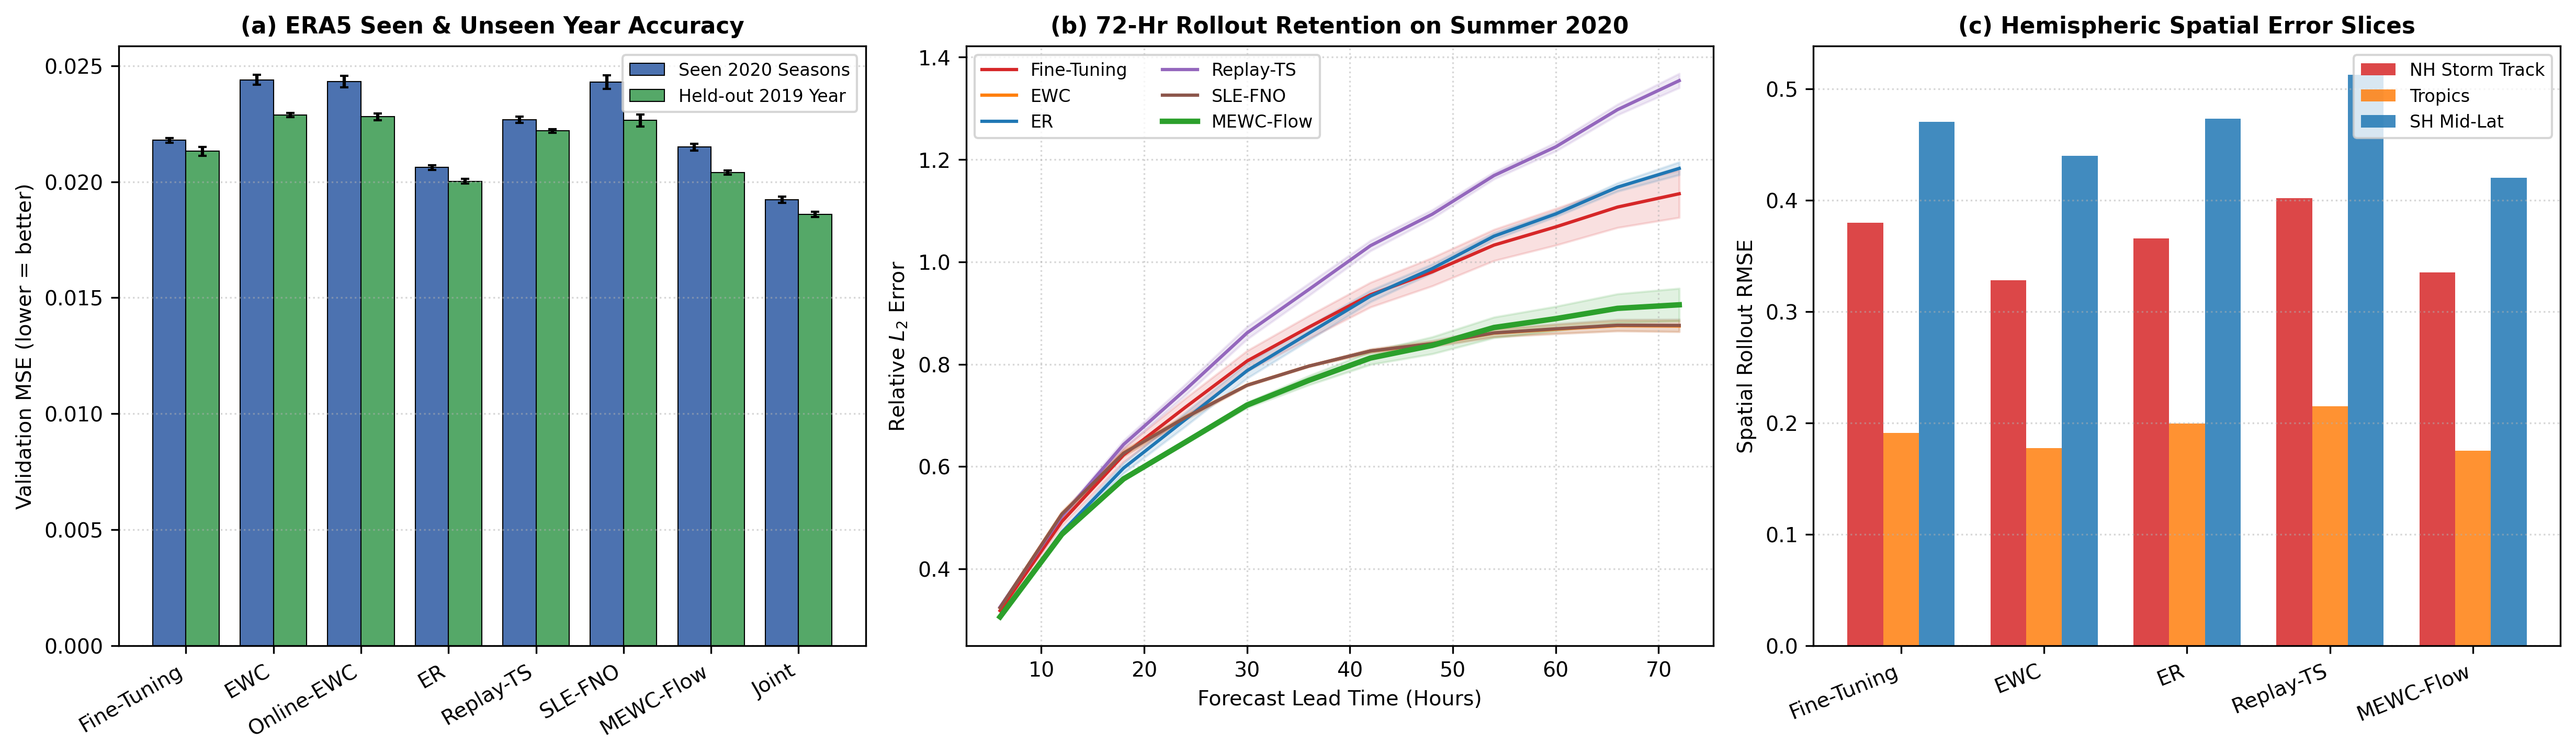
\includegraphics[width=0.96\textwidth,height=0.39\textheight,keepaspectratio]{figures/fig6_era5_planetary_analysis.png}
\caption{ERA5 seasonal wind benchmark: (a) seasonal 2020 vs.\ held-out 2019 MSE; (b) 72-h rollout stability; (c) NH mid-latitude storm-track RMSE.}
\label{fig:era5}
\end{figure}

\FloatBarrier
\subsection{Benchmark 4: 1D Viscous Burgers Shock Sequence, RQ4 \& Capacity Stress Test (3 Seeds)}

Across $\nu = 0.05 \to 0.01 \to 0.002 \to 0.0005$ (held-out $0.02, 0.005$; 20 epochs/task; $M=32$), zero-data \texttt{MEWC-PDE-Replay} ($M=0$) slashes 20-step rollout error from $0.9202$ (\texttt{Fine-Tuning}) to $0.2543$, yet anchored replay in \texttt{MEWC-Flow} reduces Final MSE by an order of magnitude to $2.37\times 10^{-5}$ and rollout error to $0.1194$ ($p=0.0011$; Table~\ref{tab:burgers}, Fig.~\ref{fig:burgers}). Under a tight capacity bottleneck (\texttt{width=16, modes=12}), \texttt{Fine-Tuning} degrades $+13{,}481.7\%$ vs.\ $+1{,}818.0\%$ for \texttt{MEWC-Flow} and $+605.1\%$ for \texttt{ER}.

\begin{table}[!htbp]
\centering
\caption{1D viscous Burgers shock steepening ($\nu = 0.05 \to 0.0005$, 3 seeds, 20 epochs/task, $M = 32$) including zero-data \texttt{MEWC-PDE-Replay} ($M = 0$).}
\label{tab:burgers}
\resizebox{\textwidth}{!}{%
\begin{tabular}{@{}lcccccc@{}}
\toprule
Method & Avg.\ Forgetting & Final MSE & Burgers PDE Residual & Rollout $t=20$ (mean of 4) & Held-out MSE & Extra MB \\
\midrule
Fine-Tuning & $2.93 \times 10^{-4} \pm 3.1 \times 10^{-5}$$^{**}$ & $2.34 \times 10^{-4} \pm 2.4 \times 10^{-5}$$^{**}$ & $4.214 \pm 0.612$ & $0.9202 \pm 0.3335$ & $2.22 \times 10^{-4} \pm 2.6 \times 10^{-5}$ & 0.000 \\
EWC & $1.66 \times 10^{-4} \pm 2.8 \times 10^{-5}$$^{*}$ & $1.53 \times 10^{-4} \pm 2.7 \times 10^{-5}$$^{*}$ & $3.851 \pm 0.697$ & $0.6873 \pm 0.1733$$^{*}$ & $1.05 \times 10^{-4} \pm 2.5 \times 10^{-6}$ & 0.634 \\
Online-EWC & $1.96 \times 10^{-4} \pm 2.8 \times 10^{-5}$$^{**}$ & $1.69 \times 10^{-4} \pm 2.4 \times 10^{-5}$$^{**}$ & $3.912 \pm 0.699$ & $0.7381 \pm 0.2014$$^{*}$ & $1.29 \times 10^{-4} \pm 1.1 \times 10^{-5}$ & 0.634 \\
ER & $-2.13 \times 10^{-6} \pm 2.5 \times 10^{-6}$ & $1.73 \times 10^{-5} \pm 4.6 \times 10^{-7}$ & $2.943 \pm 0.608$ & $0.0780 \pm 0.0047$ & $1.13 \times 10^{-5} \pm 1.9 \times 10^{-6}$ & 0.133 \\
Replay-TS & $-3.35 \times 10^{-6} \pm 1.3 \times 10^{-6}$ & $1.82 \times 10^{-5} \pm 3.2 \times 10^{-6}$ & $2.977 \pm 0.608$ & $0.0839 \pm 0.0125$ & $1.17 \times 10^{-5} \pm 3.7 \times 10^{-6}$ & 0.129 \\
SLE-FNO & $-3.08 \times 10^{-7} \pm 7.4 \times 10^{-7}$ & $1.99 \times 10^{-4} \pm 4.4 \times 10^{-5}$$^{*}$ & $4.206 \pm 0.722$ & $0.3077 \pm 0.0259$$^{*}$ & $1.94 \times 10^{-4} \pm 1.2 \times 10^{-5}$ & 0.010 \\
MEWC-PDE-Replay ($M=0$) & $1.41 \times 10^{-4} \pm 6.5 \times 10^{-5}$ & $1.28 \times 10^{-4} \pm 4.7 \times 10^{-5}$ & $3.702 \pm 0.818$ & $0.2543 \pm 0.0194$$^{**}$ & $1.24 \times 10^{-4} \pm 3.1 \times 10^{-5}$ & 1.059 \\
\textbf{MEWC-Flow} & $\mathbf{4.49 \times 10^{-6} \pm 5.2 \times 10^{-6}}$ & $\mathbf{2.37 \times 10^{-5} \pm 3.3 \times 10^{-6}}$ & $\mathbf{3.015 \pm 0.591}$ & $\mathbf{0.1194 \pm 0.0270}$ & $\mathbf{2.94 \times 10^{-5} \pm 9.0 \times 10^{-6}}$ & \textbf{1.277} \\
Joint & $0.00 \times 10^{0} \pm 0.0 \times 10^{0}$ & $9.48 \times 10^{-6} \pm 1.0 \times 10^{-6}$$^{*}$ & $2.852 \pm 0.570$ & $0.0551 \pm 0.0045$$^{*}$ & $3.89 \times 10^{-6} \pm 1.1 \times 10^{-6}$ & 3.834 \\
\bottomrule
\end{tabular}%
}
\end{table}

\begin{figure}[!htbp]
\centering
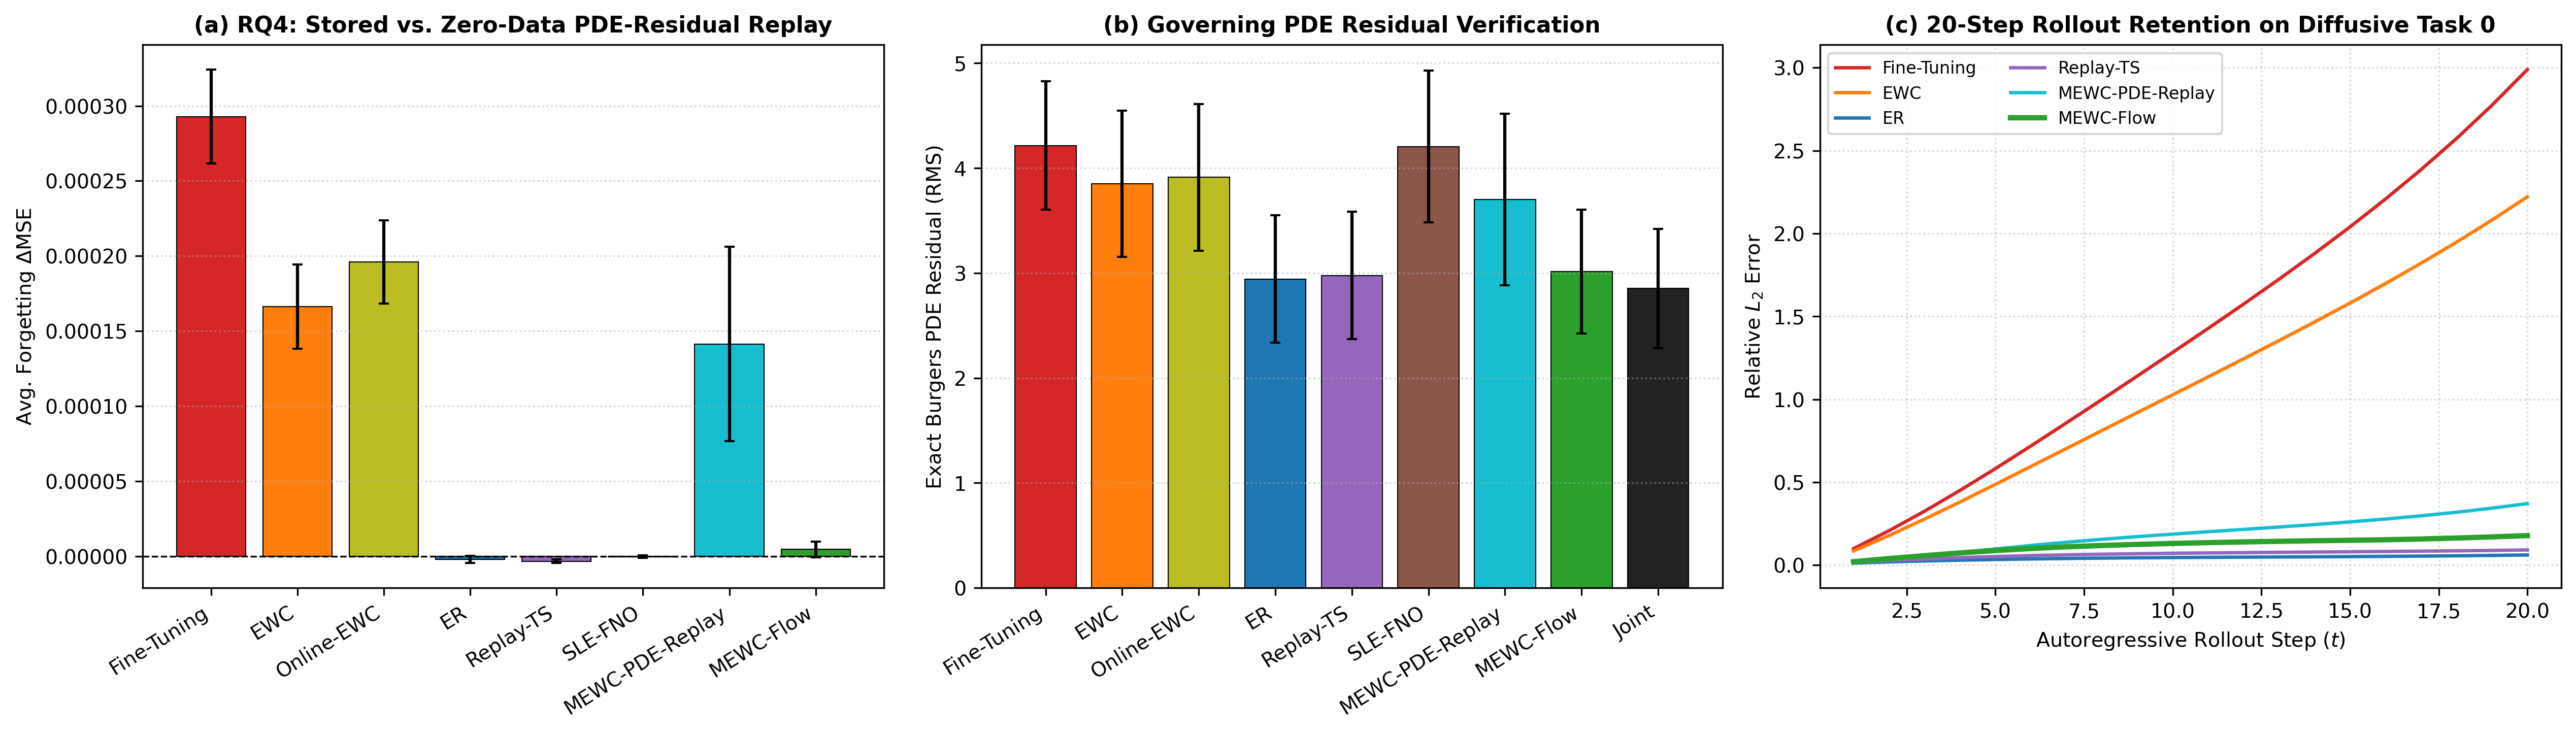
\includegraphics[width=0.96\textwidth,height=0.39\textheight,keepaspectratio]{figures/fig7_burgers_pde_residual_replay.png}
\caption{1D viscous Burgers shock sequence ($\nu=0.05 \to 0.0005$) and RQ4 zero-data PDE replay comparison.}
\label{fig:burgers}
\end{figure}

\FloatBarrier
\subsection{Neuro-Fuzzy Head-to-Head Benchmark (\texttt{Fuzzy-MEWC-Flow} vs.\ Neural \texttt{MEWC-Flow})}

Comparing \texttt{Fuzzy-MEWC-Flow} against neural \texttt{MEWC-Flow} across all 4 multi-seed benchmarks (Table~\ref{tab:fuzzy}, Fig.~\ref{fig:neuro_fuzzy}): on 2D wakes (PIV) and Navier--Stokes bifurcations (Kolmogorov), the interpretable 5-invariant ANFIS router + 9-rule Sugeno controller matches neural \texttt{MEWC-Flow} within statistical noise on Final MSE ($p=0.2217$) and NS PDE residual ($7.039$ vs.\ $7.040$, $p=0.9950$), while on real ERA5 planetary winds it sets the best 72-h rollout ($0.9170 \pm 0.0181$, beating \texttt{ER} at $p=0.0030$) and NH storm-track RMSE ($0.3317$). On 1D Burgers shocks, scalar Gaussian rules trade some shock precision ($6.45\times 10^{-5}$ vs.\ $2.37\times 10^{-5}$ MSE) for transparent IF--THEN interpretability (seed-0 PIV silhouette $0.777$, held-out $Re=910^* \to [0.00, 0.03, 0.91, 0.06]$ and $Re=1890^* \to [0.00, 0.00, 0.03, 0.97]$).

\begin{table}[!htbp]
\centering
\caption{Neuro-Fuzzy \texttt{Fuzzy-MEWC-Flow} vs.\ Neural \texttt{MEWC-Flow} across all four multi-seed benchmarks.}
\label{tab:fuzzy}
\resizebox{\textwidth}{!}{%
\begin{tabular}{@{}llccccc@{}}
\toprule
Benchmark & Variant & Avg.\ Forgetting & Final MSE & Key Physics / Rollout Metric & Held-out / RegID & Extra MB \\
\midrule
PIV (5 seeds) & MEWC-Flow (Neural) & $-7.78 \times 10^{-5} \pm 1.8 \times 10^{-5}$ & $1.05 \times 10^{-3} \pm 1.7 \times 10^{-5}$ & R10 $= 0.0997 \pm 0.0053$ / Vort $= 0.0278 \pm 0.0020$ & RegAcc $= 0.776 \pm 0.046$ & 10.32 \\
PIV (5 seeds) & \textbf{Fuzzy-MEWC-Flow} & $\mathbf{-6.96 \times 10^{-5} \pm 2.4 \times 10^{-5}}$ & $\mathbf{1.05 \times 10^{-3} \pm 2.1 \times 10^{-5}}$ & $\mathbf{\text{R10} = 0.1011 \pm 0.0021}$ / $\mathbf{\text{Vort} = 0.0282 \pm 0.0009}$ & $\mathbf{\text{RegAcc} = 0.634 \pm 0.002}$ & \textbf{10.15} \\
\midrule
Kolmogorov NS (3 seeds) & MEWC-Flow (Neural) & $-1.00 \times 10^{-3} \pm 1.3 \times 10^{-4}$ & $3.31 \times 10^{-3} \pm 1.8 \times 10^{-4}$ & NS\_PDE $= 7.040 \pm 0.017$ / R10 $= 0.3442 \pm 0.0092$ & HO $= 4.80 \times 10^{-3} \pm 2.7 \times 10^{-4}$ & 10.32 \\
Kolmogorov NS (3 seeds) & \textbf{Fuzzy-MEWC-Flow} & $\mathbf{-1.02 \times 10^{-3} \pm 1.5 \times 10^{-4}}$ & $\mathbf{3.42 \times 10^{-3} \pm 1.6 \times 10^{-4}}$ & $\mathbf{\text{NS\_PDE} = 7.039 \pm 0.030}$ / $\mathbf{\text{R10} = 0.3499 \pm 0.0116}$ & $\mathbf{\text{HO} = 4.85 \times 10^{-3} \pm 2.0 \times 10^{-4}}$ & \textbf{10.15} \\
\midrule
ERA5 Winds (3 seeds) & MEWC-Flow (Neural) & $-1.29 \times 10^{-3} \pm 1.4 \times 10^{-4}$ & $2.15 \times 10^{-2} \pm 1.5 \times 10^{-4}$ & R72h $= 0.9260 \pm 0.0149$ / NH $= 0.3352 \pm 0.0036$ & HO\_Sum $= 2.01 \times 10^{-2} \pm 1.0 \times 10^{-4}$ & 8.22 \\
ERA5 Winds (3 seeds) & \textbf{Fuzzy-MEWC-Flow} & $\mathbf{-1.26 \times 10^{-3} \pm 1.7 \times 10^{-4}}$ & $\mathbf{2.17 \times 10^{-2} \pm 1.0 \times 10^{-4}}$ & $\mathbf{\text{R72h} = 0.9170 \pm 0.0181}$ / $\mathbf{\text{NH} = 0.3317 \pm 0.0026}$ & $\mathbf{\text{HO\_Sum} = 2.03 \times 10^{-2} \pm 5.7 \times 10^{-5}}$ & \textbf{8.06} \\
\midrule
Burgers 1D (3 seeds) & MEWC-Flow (Neural) & $+4.49 \times 10^{-6} \pm 5.2 \times 10^{-6}$ & $2.37 \times 10^{-5} \pm 3.3 \times 10^{-6}$ & PDE $= 3.015 \pm 0.591$ / R20 $= 0.1194 \pm 0.0270$ & HO $= 2.94 \times 10^{-5} \pm 9.0 \times 10^{-6}$ & 1.277 \\
Burgers 1D (3 seeds) & \textbf{Fuzzy-MEWC-Flow} & $\mathbf{+4.44 \times 10^{-5} \pm 2.2 \times 10^{-5}}$ & $\mathbf{6.45 \times 10^{-5} \pm 2.1 \times 10^{-5}}$ & $\mathbf{\text{PDE} = 3.462 \pm 0.724}$ / $\mathbf{\text{R20} = 0.2370 \pm 0.0733}$ & $\mathbf{\text{HO} = 6.44 \times 10^{-5} \pm 6.5 \times 10^{-6}}$ & \textbf{1.192} \\
\bottomrule
\end{tabular}%
}
\end{table}

\begin{figure}[!htbp]
\centering
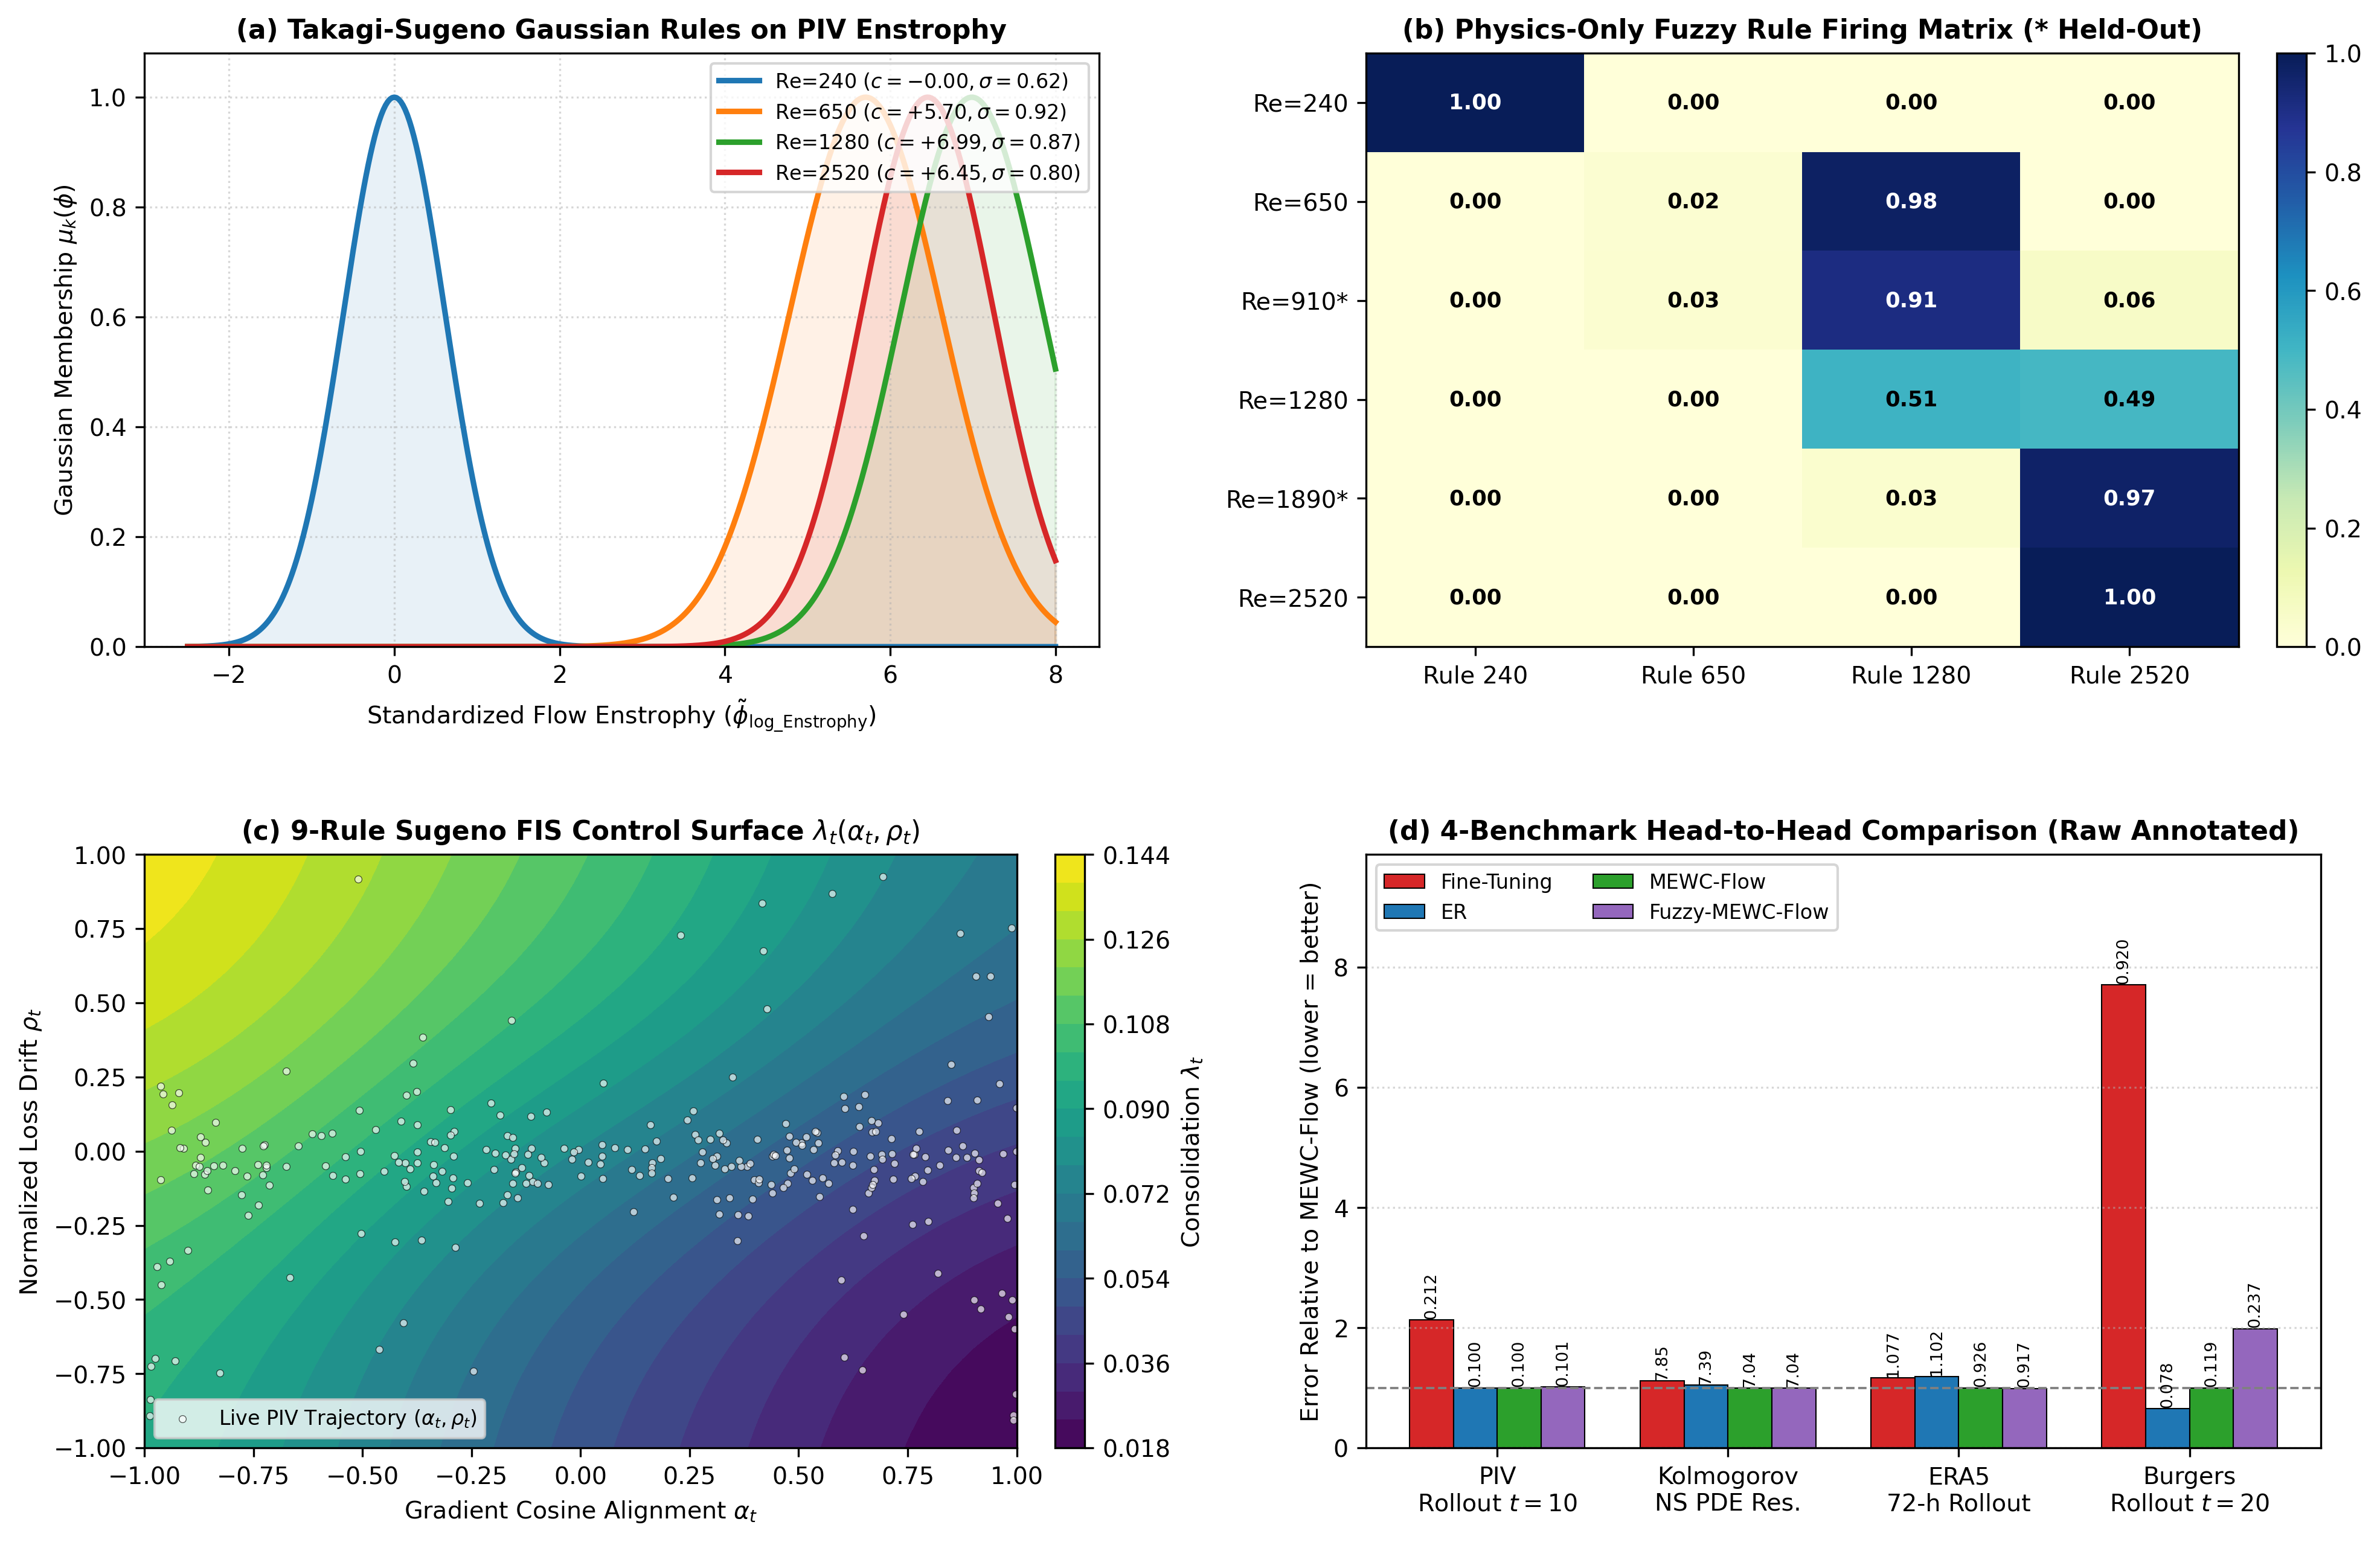
\includegraphics[width=0.96\textwidth,height=0.39\textheight,keepaspectratio]{figures/fig8_neuro_fuzzy_interpretability.png}
\caption{Neuro-Fuzzy \texttt{Fuzzy-MEWC-Flow} interpretability: (a) learned ANFIS Gaussian memberships; (b) zero-leakage rule firing matrix; (c) 9-rule Sugeno $\lambda_t(\alpha_t, \rho_t)$ control surface; (d) 4-benchmark summary.}
\label{fig:neuro_fuzzy}
\end{figure}

% ==============================================================================
\section{Our Six-Layer Error Analysis \& Verification Process}
% ==============================================================================

Because single-step pixel MSE routinely hides unphysical divergence, high-wavenumber spectral collapse, or autoregressive blowup, we built a \textbf{six-layer error analysis and automated verification pipeline}:

\begin{enumerate}
  \item \textbf{Continual Retention \& Transfer Matrix Audit:} Full $K\times K$ matrix $E_{i,j}$ computation separating forward transfer, backward forgetting ($-\text{BWT}$), Task-0 degradation (\%), and unseen held-out regime interpolation.
  \item \textbf{Multi-Window Autoregressive Rollouts \& $\text{VPH}_{0.25}$:} Evaluating recursive error growth across 10--20 steps (fluid wakes/NS/Burgers) and 72-h atmospheric forecasts (ERA5) alongside $\text{VPH}_{0.25}$, exposing rollout blowup in \texttt{ER}/\texttt{Replay-TS} on ERA5 ($1.1024$--$1.2253$) vs.\ \texttt{MEWC-Flow} ($0.9260$).
  \item \textbf{Physical Invariant, Governing PDE Residual \& Spectral Band Decomposition:} Auditing finite-difference vorticity RMSE, $\|\nabla\cdot\mathbf{u}\|_{\text{RMS}}$, exact 2D NS and 1D Burgers PDE residuals, kinetic energy/enstrophy errors, and radial spectra $E(k)$ decomposed into low-, mid- (inertial), and high-wavenumber bands (\texttt{physics\_and\_rollout\_summary.json}).
  \item \textbf{Zero-Leakage Latent Manifold \& Routing Failure Audit:} Computing PCA variance, silhouette score ($0.518$ seed-0), and confusion matrices without $Re$ input, confirming that all routing errors on PIV concentrate in the physical shedding transition ($Re=650 \leftrightarrow 1280$).
  \item \textbf{Component Ablations, Curriculum Ordering \& Byte-Level Memory Pareto Sweeps (Tables~\ref{tab:ablation}--\ref{tab:memory}, Fig.~\ref{fig:piv_ablations}):} Removing episodic replay ($0\text{ MB}$) doubles Task-0 rollout error ($0.0985 \to 0.2248$), proving replay is the dominant PIV anti-forgetting driver; ascending $Re$ curriculum inflicts $+4.12\times 10^{-4}$ forgetting on \texttt{Fine-Tuning} vs.\ $-4.48\times 10^{-5}$ descending, while \texttt{MEWC-Flow} maintains negative forgetting under all orders and scales monotonically from $M=4$ to $M=32$.
  \item \textbf{Statistical Significance \& Strict-JSON Programmatic Verification:} Paired two-sided $t$-tests ($p$) and Cohen's $d$ across matched random seeds (\texttt{mewc\_flow/utils/stats.py}), strict-JSON checks (\texttt{allow\_nan=False}), and automated manuscript table verification via \texttt{tests/test\_verification.py}, \texttt{tests/build\_manuscript\_tables.py}, and \texttt{tests/\allowbreak verify\_\allowbreak manuscript\_\allowbreak numbers.py}.
\end{enumerate}

\begin{table}[!htbp]
\centering
\caption{Systematic PIV component ablation across 3 seeds (\texttt{42, 102, 202}, 12 epochs/task).}
\label{tab:ablation}
\resizebox{\textwidth}{!}{%
\begin{tabular}{@{}lcccccc@{}}
\toprule
Variant & Avg.\ Forgetting & Final MSE & Rollout $t=10$ & Vorticity RMSE & Held-out MSE & Extra MB \\
\midrule
Full MEWC-Flow & $-9.80 \times 10^{-5} \pm 1.3 \times 10^{-5}$ & $1.08 \times 10^{-3} \pm 8.3 \times 10^{-6}$ & $0.0985 \pm 0.0043$ & $0.0273 \pm 0.0021$ & $1.31 \times 10^{-3} \pm 1.6 \times 10^{-5}$ & 10.32 \\
w/o Modular Adapters & $-1.14 \times 10^{-4} \pm 1.1 \times 10^{-5}$ & $1.06 \times 10^{-3} \pm 4.6 \times 10^{-6}$ & $0.0961 \pm 0.0026$ & $0.0263 \pm 0.0014$ & $1.28 \times 10^{-3} \pm 5.4 \times 10^{-6}$ & 10.31 \\
w/o Contrastive Router & $-9.83 \times 10^{-5} \pm 8.2 \times 10^{-6}$ & $1.09 \times 10^{-3} \pm 5.7 \times 10^{-6}$ & $0.0965 \pm 0.0036$ & $0.0265 \pm 0.0017$ & $1.31 \times 10^{-3} \pm 1.2 \times 10^{-5}$ & 10.15 \\
w/o Adaptive EWC (Static) & $-9.54 \times 10^{-5} \pm 9.3 \times 10^{-6}$ & $1.10 \times 10^{-3} \pm 2.9 \times 10^{-6}$ & $0.0976 \pm 0.0039$ & $0.0268 \pm 0.0018$ & $1.33 \times 10^{-3} \pm 1.1 \times 10^{-5}$ & 7.94 \\
w/o EWC & $-9.38 \times 10^{-5} \pm 1.4 \times 10^{-5}$ & $1.07 \times 10^{-3} \pm 1.1 \times 10^{-5}$ & $0.0987 \pm 0.0042$ & $0.0274 \pm 0.0019$ & $1.30 \times 10^{-3} \pm 1.7 \times 10^{-5}$ & 4.37 \\
w/o Episodic Replay (0 MB) & $+4.28 \times 10^{-4} \pm 7.1 \times 10^{-4}$ & $1.50 \times 10^{-3} \pm 5.3 \times 10^{-4}$ & $0.2248 \pm 0.0763$ & $0.0319 \pm 0.0025$ & $1.59 \times 10^{-3} \pm 3.4 \times 10^{-4}$ & 6.12 \\
w/o Physics Loss & $-9.93 \times 10^{-5} \pm 1.3 \times 10^{-5}$ & $1.08 \times 10^{-3} \pm 7.5 \times 10^{-6}$ & $0.0982 \pm 0.0044$ & $0.0272 \pm 0.0021$ & $1.31 \times 10^{-3} \pm 1.5 \times 10^{-5}$ & 10.32 \\
Replay-Only (ER) & $-1.09 \times 10^{-4} \pm 7.0 \times 10^{-6}$ & $1.07 \times 10^{-3} \pm 1.1 \times 10^{-5}$ & $0.0953 \pm 0.0030$ & $0.0263 \pm 0.0020$ & $1.29 \times 10^{-3} \pm 1.3 \times 10^{-5}$ & 4.20 \\
\bottomrule
\end{tabular}%
}
\end{table}

\begin{table}[!htbp]
\centering
\caption{Routing mode ablation on Full MEWC-Flow (3 seeds). Soft and hard learned routing match ground-truth oracle routing and outperform uniform averaging.}
\label{tab:routing_modes}
\begin{tabular}{@{}lccc@{}}
\toprule
Routing Mode & Seen Final MSE & Held-out MSE & Rollout $t=10$ \\
\midrule
\texttt{soft} & $1.08 \times 10^{-3} \pm 8.3 \times 10^{-6}$ & $1.31 \times 10^{-3} \pm 1.6 \times 10^{-5}$ & $0.0985 \pm 0.0043$ \\
\texttt{hard} & $1.08 \times 10^{-3} \pm 8.7 \times 10^{-6}$ & $1.31 \times 10^{-3} \pm 1.6 \times 10^{-5}$ & $0.0985 \pm 0.0043$ \\
\texttt{uniform} & $1.09 \times 10^{-3} \pm 1.3 \times 10^{-5}$ & $1.31 \times 10^{-3} \pm 1.5 \times 10^{-5}$ & $0.1003 \pm 0.0048$ \\
\texttt{oracle} & $1.08 \times 10^{-3} \pm 7.9 \times 10^{-6}$ & -- & $0.0985 \pm 0.0043$ \\
\bottomrule
\end{tabular}
\end{table}

\begin{table}[!htbp]
\centering
\caption{Task-order sensitivity across ascending ($240 \to 2520$), descending ($2520 \to 240$), and shuffled ($1280 \to 240 \to 2520 \to 650$) curricula (RQ5, 3 seeds, Avg.\ Forgetting / Final MSE).}
\label{tab:order}
\resizebox{\textwidth}{!}{%
\begin{tabular}{@{}lccc@{}}
\toprule
Curriculum Order & Fine-Tuning & ER & MEWC-Flow \\
\midrule
Ascending ($240 \to 2520$) & $+4.12 \times 10^{-4} \pm 5.7 \times 10^{-4}$ / $1.46 \times 10^{-3}$ & $-1.09 \times 10^{-4} \pm 7.0 \times 10^{-6}$ / $1.07 \times 10^{-3}$ & $-9.80 \times 10^{-5} \pm 1.3 \times 10^{-5}$ / $1.08 \times 10^{-3}$ \\
Descending ($2520 \to 240$) & $-4.48 \times 10^{-5} \pm 5.0 \times 10^{-5}$ / $1.22 \times 10^{-3}$ & $-2.24 \times 10^{-4} \pm 3.0 \times 10^{-6}$ / $1.06 \times 10^{-3}$ & $-1.46 \times 10^{-4} \pm 1.4 \times 10^{-5}$ / $1.16 \times 10^{-3}$ \\
Shuffled ($1280 \to 240 \to 2520 \to 650$) & $+2.57 \times 10^{-5} \pm 5.6 \times 10^{-5}$ / $1.22 \times 10^{-3}$ & $-1.24 \times 10^{-4} \pm 7.8 \times 10^{-6}$ / $1.07 \times 10^{-3}$ & $-1.07 \times 10^{-4} \pm 6.9 \times 10^{-6}$ / $1.13 \times 10^{-3}$ \\
\bottomrule
\end{tabular}%
}
\end{table}

\begin{table}[!htbp]
\centering
\caption{Episodic memory-budget scaling ($M \in \{4, 8, 16, 32\}$ exemplars/task, step-10 rollout rel-$L_2$ / extra CL MB).}
\label{tab:memory}
\begin{tabular}{@{}cccc@{}}
\toprule
$M$ per task & ER & Replay-TS & MEWC-Flow \\
\midrule
4 & 0.1214 / 1.05 MB & 0.1266 / 0.79 MB & 0.1239 / 7.17 MB \\
8 & 0.1045 / 2.10 MB & 0.1184 / 1.97 MB & 0.1064 / 8.22 MB \\
16 & 0.0953 / 4.20 MB & 0.0936 / 3.93 MB & 0.0985 / 10.32 MB \\
32 & 0.0957 / 8.39 MB & 0.0904 / 8.26 MB & 0.0954 / 14.51 MB \\
\bottomrule
\end{tabular}
\end{table}

\begin{figure}[!htbp]
\centering
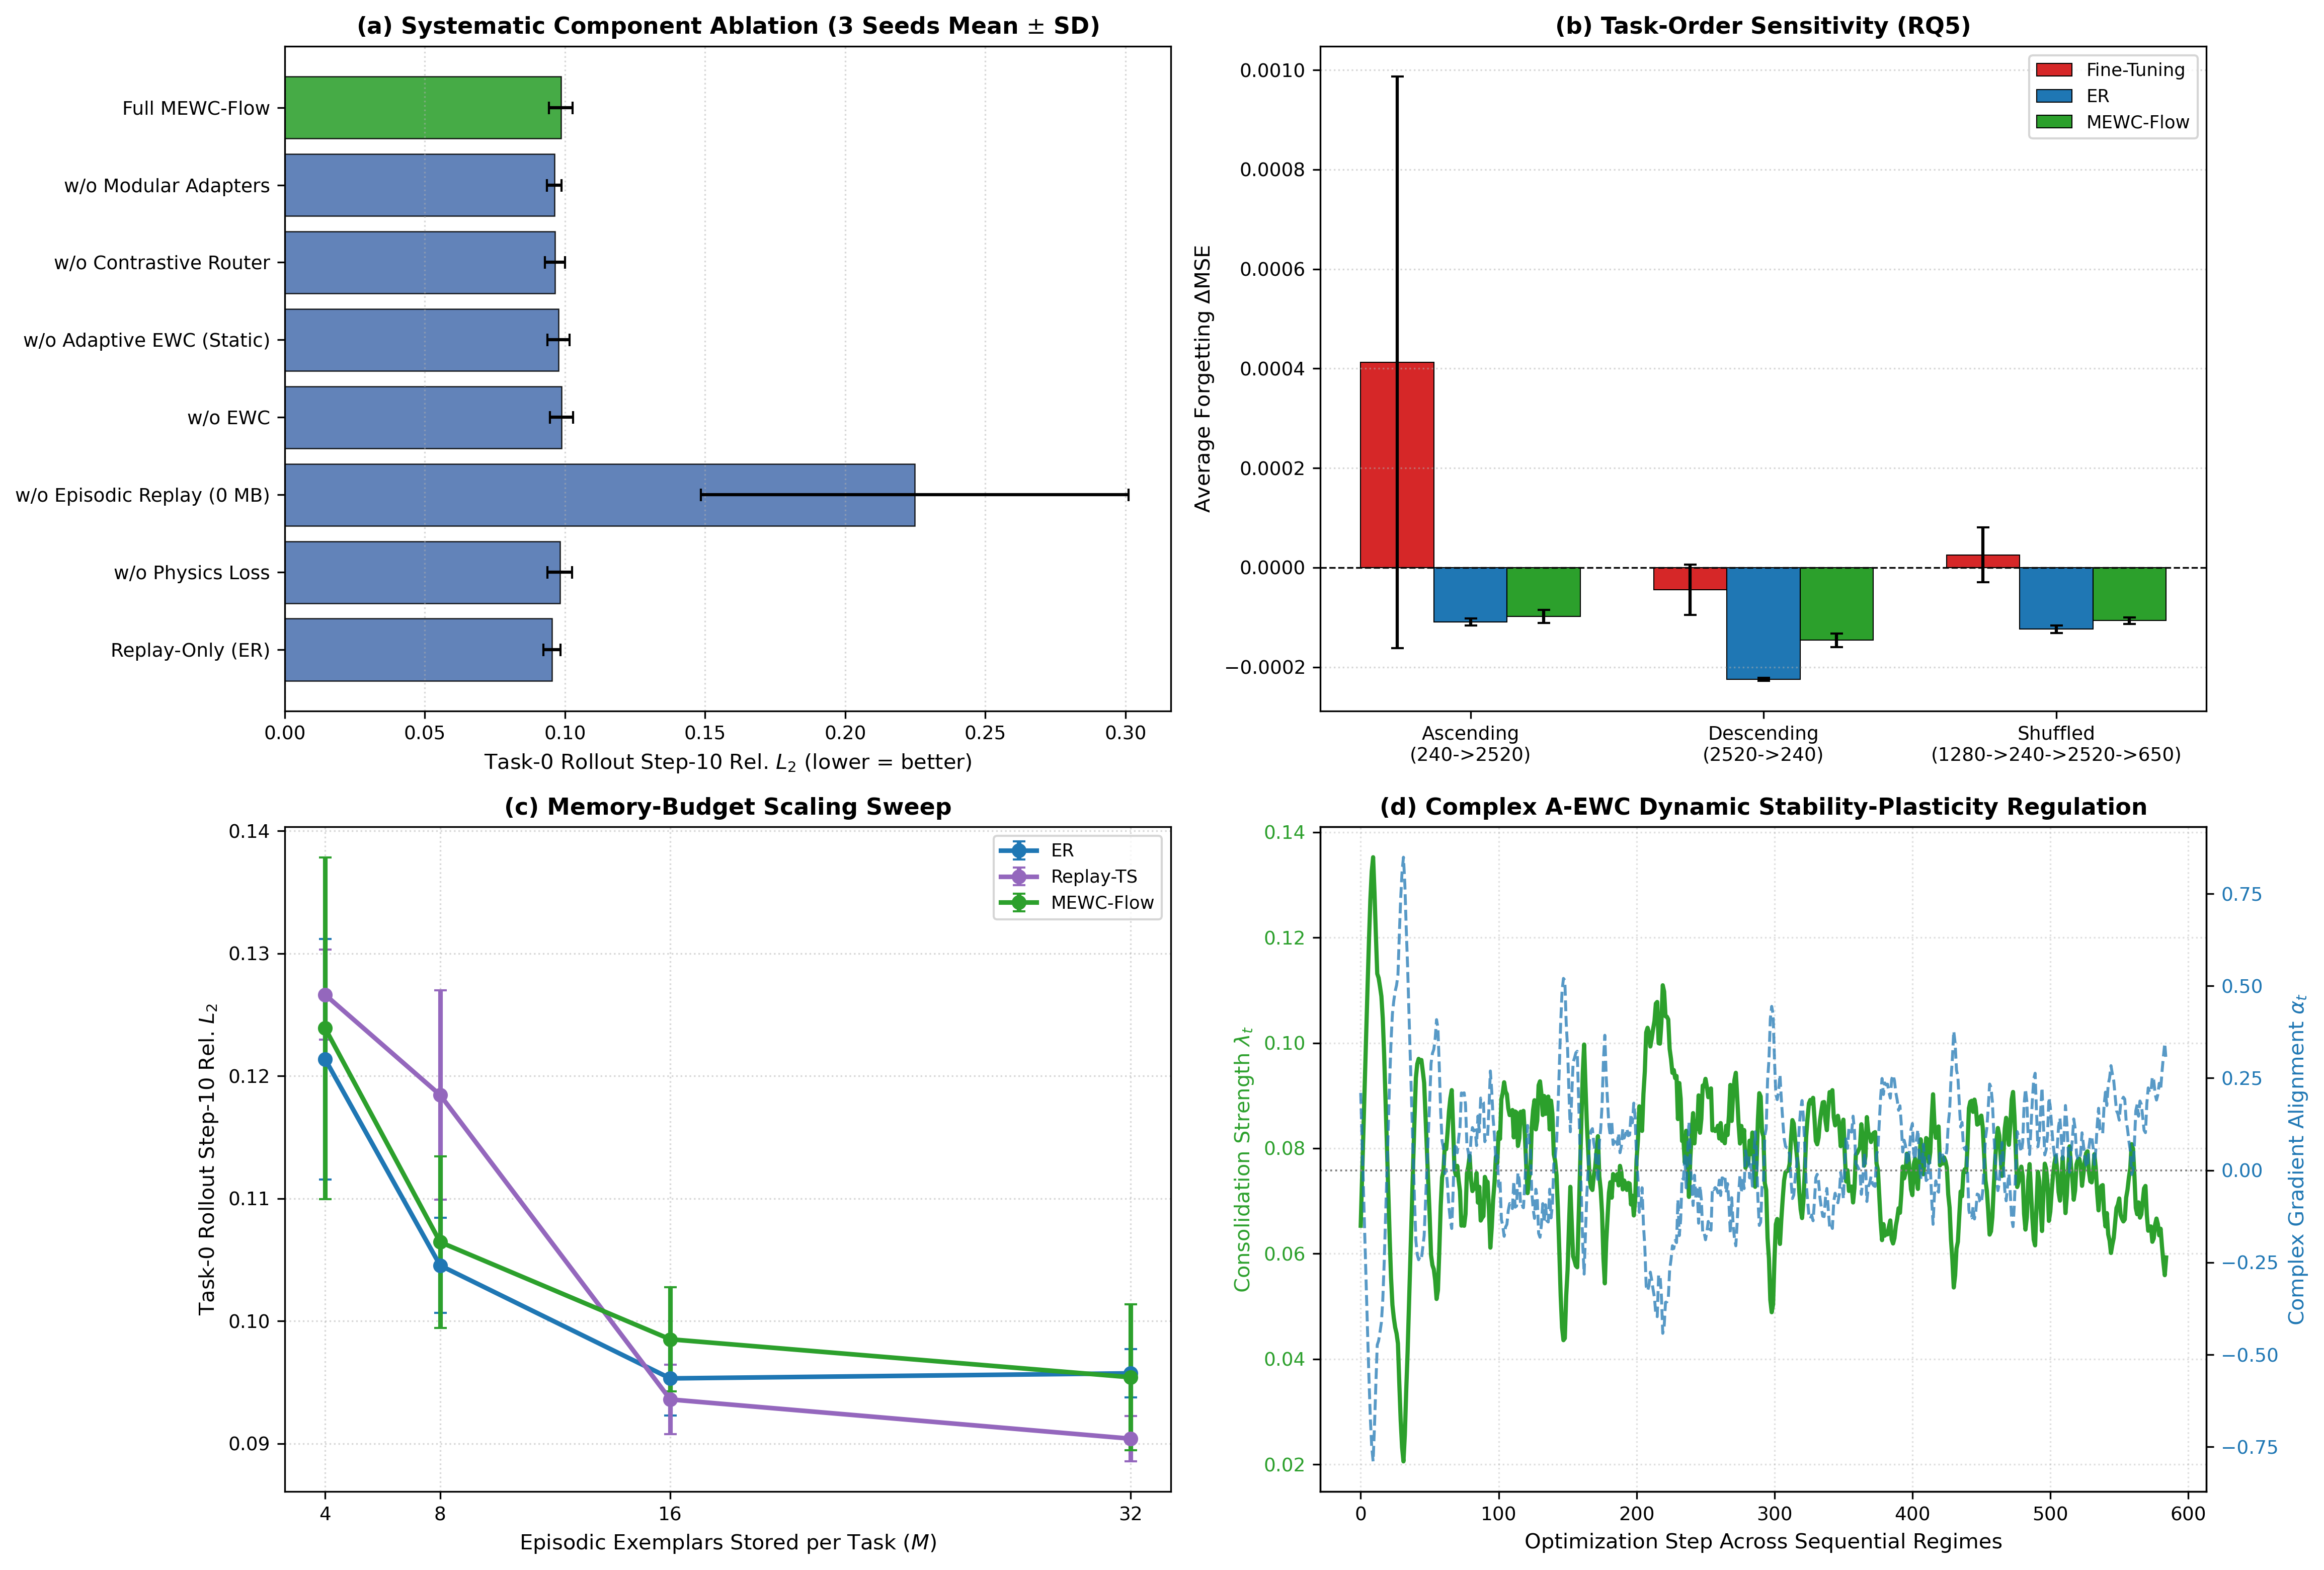
\includegraphics[width=0.96\textwidth,height=0.39\textheight,keepaspectratio]{figures/fig4_piv_ablations_and_sensitivity.png}
\caption{(a) Component ablation confirming episodic replay dominance on PIV rollout stability; (b) curriculum order sensitivity; (c) memory scaling; (d) live Complex A-EWC $\alpha_t \to \lambda_t$ trace.}
\label{fig:piv_ablations}
\end{figure}

% ==============================================================================
\section{Synthesis of RQ1--RQ5, Candid Limitations \& Supervisor Review Points}
% ==============================================================================

\begin{itemize}
  \item \textbf{RQ1:} Episodic replay drives anti-forgetting on stationary geometries, while complex A-EWC + adapters preserve stability across all four benchmarks ($-7.78\times 10^{-5}$ PIV, $-1.00\times 10^{-3}$ NS, $-1.29\times 10^{-3}$ ERA5, $+4.49\times 10^{-6}$ Burgers).
  \item \textbf{RQ2:} Low 1-step MSE $\neq$ physical fidelity. \texttt{MEWC-Flow} leads on exact 2D NS PDE residual ($7.040$, $p\le 0.015$ vs.\ all baselines including \texttt{Joint}), PIV inertial spectrum ($0.0484$), and ERA5 72-h rollouts ($0.9260$ vs.\ \texttt{ER} $1.1024$).
  \item \textbf{RQ3:} Zero-leakage physics-only routing reaches $77.6\% \pm 4.6\%$ ($84.2\%$ seed-0), matches oracle routing ($1.08\times 10^{-3}$), and smoothly interpolates held-out $Re=910^*, 1890^*$.
  \item \textbf{RQ4:} Zero-data PDE replay (\texttt{MEWC-PDE-Replay}) cuts Burgers rollout error fourfold ($0.9202 \to 0.2543$) without stored snapshots, yet sample-anchored replay remains essential under $100\times$ viscosity shocks ($0.078$--$0.119$).
  \item \textbf{RQ5:} Ascending $Re$ order breaks \texttt{Fine-Tuning} ($+4.12\times 10^{-4}$), whereas \texttt{MEWC-Flow} stays negative-forgetting across all permutations and scales cleanly from $M=4$ to $M=32$.
\end{itemize}

\subsection*{Candid Limitations \& Decisions Requested from Supervisor}
\begin{enumerate}
  \item \textbf{Memory \& 1-Step MSE Trade-off vs.\ Monolithic \texttt{ER}:} \texttt{MEWC-Flow} adds $\approx 6.1\text{ MB}$ parameter/Fisher overhead over equal-$M$ \texttt{ER} and trails \texttt{ER} slightly on 1-step MSE in steady-geometry Burgers ($2.37\times 10^{-5}$ vs.\ $1.73\times 10^{-5}$) and Kolmogorov NS ($3.31\times 10^{-3}$ vs.\ $2.99\times 10^{-3}$), excelling instead on \emph{PDE consistency, zero-label regime routing, and multi-step atmospheric rollouts}.
  \item \textbf{Items for Supervisor Sign-Off:}
  \begin{itemize}
    \item \emph{Target Q1 Journal Selection:} Confirm preferred venue (e.g., \textit{Journal of Computational Physics}, \textit{Computer Methods in Applied Mechanics and Engineering}, or \textit{Journal of Machine Learning for Modeling and Computing}) to finalize journal template formatting.
    \item \emph{Scope of Transitional Overlap ($Re=650 \leftrightarrow 1280$):} Confirm whether reporting single-snapshot routing ($84.2\%$ seed-0) alongside physical Strouhal overlap explanation suffices, or whether a multi-frame temporal pooling ablation should be added before submission.
    \item \emph{3D Extension Scope:} Confirm treating 3D volumetric LES/DNS velocity fields explicitly as future work given the current 4-benchmark scope (PIV, Kolmogorov NS, ERA5, Burgers).
  \end{itemize}
\end{enumerate}

% ==============================================================================
\FloatBarrier
\begin{thebibliography}{99}

\bibitem{wang2026replay}
Wang, Y.-Z., Eshaghi, M., Zhuang, X.-Y., Rabczuk, T., \& Liu, Y.-H. (2026). Replay-Based Continual Learning for Physics-Informed Neural Operators. \textit{arXiv:2605.04832}. \url{https://doi.org/10.48550/arXiv.2605.04832}

\bibitem{elhadidy2026slefno}
Elhadidy, M., D'Souza, R. M., \& Arzani, A. (2026). SLE-FNO: Single-layer extensions for task-agnostic continual learning in Fourier neural operators. \textit{Physica Scripta}. \url{https://doi.org/10.1088/1402-4896/ae6bdd}

\bibitem{hemati2026replayts}
Hemati, H., Nguyen, B. D., \& Sandfeld, S. (2026). Continual learning for autoregressive PDE surrogates under evolving physical regimes. \textit{Machine Learning for Computational Science and Engineering}. \url{https://doi.org/10.1007/s44379-026-00085-9}

\bibitem{ji2026pmoe}
Ji, H.-Y., Luo, Y., Zhou, H., \& Zhao, Y. (2026). Progressive mixture-of-experts with autoencoder routing for continual RANS turbulence modelling. \textit{Journal of Fluid Mechanics}. \url{https://doi.org/10.1017/jfm.2026.11654}

\bibitem{winkler2026nfl}
Winkler, G., \& Stoll, M. (2026). No Free Lunch in Flow Surrogates under Time-Varying Boundary Conditions: A Two-Regime Study. \textit{Journal of Computational Science}.

\bibitem{kim2026mgann}
Kim, M.-S., Mo, H. S., Lacey, C. E., Jung, K.-S., Chen, J. H., \& Yoo, C. (2026). MG-ANN: An online extension of reduced-order modeling with continual learning for turbulent reacting flows. \textit{Proceedings of the Combustion Institute}. \url{https://doi.org/10.1016/j.proci.2026.106546}

\bibitem{chen2026clpinn}
Chen, X.-J., Hu, X., Chen, L., Liu, Y., \& Fan, W. (2026). Continual-Learning Physics-Informed Neural Networks for Parameterized Partial Differential Equations. \textit{arXiv preprint}.

\bibitem{howard2023multifidelity}
Howard, A. A., Fu, Y., \& Stinis, P. (2023). A multifidelity approach to continual learning for physical systems. \textit{Machine Learning: Science and Technology}, 4, 025042. \url{https://doi.org/10.1088/2632-2153/ad45b2}

\bibitem{guo2026renanet}
Guo, Y., Qiang, Y.-M., Chu, X., Ding, J., Chen, Y., Wang, Q., Wu, T., \& Zhang, A. (2026). RenaNet: Reynolds-Aware Neural Network for Rapid Flow Field Prediction via Lattice Boltzmann Simulations. \textit{Applied Sciences}, 16(13), 6622. \url{https://doi.org/10.3390/app16136622}

\bibitem{shi2026striding}
Shi, J. (2026). Striding Across Reynolds Numbers: Representation Geometry in Neural PDE Generalisation. \textit{arXiv:2605.30112}. \url{https://doi.org/10.48550/arXiv.2605.30112}

\bibitem{dekhovich2025ipinns}
Dekhovich, A., Sluiter, M. H. F., Tax, D. M. J., \& Bessa, M. A. (2025). iPINNs: incremental learning for Physics-informed neural networks. \textit{Engineering with Computers}, 41, 389--402. \url{https://doi.org/10.1007/s00366-024-02010-1}

\bibitem{kirkpatrick2017ewc}
Kirkpatrick, J., Pascanu, R., Rabinowitz, N., Veness, J., Desjardins, G., Rusu, A. A., et al. (2017). Overcoming catastrophic forgetting in neural networks. \textit{Proceedings of the National Academy of Sciences (PNAS)}, 114(13), 3521--3526. \url{https://doi.org/10.1073/pnas.1611835114}

\bibitem{lagemann2026hydrogym}
Lagemann, C., Paehler, L., Callaham, J. L., Mokbel, S., Ahnert, S., Lagemann, K., Adams, N. A., Vinuesa, R., \& Brunton, S. L. (2026). The HydroGym Reinforcement Learning Platform for Fluid Dynamics. \textit{Nature}.

\bibitem{schwarz2018onlineewc}
Schwarz, J., Luketina, J., Czarnecki, W. M., Grabska-Barwinska, A., Teh, Y. W., Pascanu, R., \& Hadsell, R. (2018). Progress \& Compress: A scalable framework for continual learning. \textit{Proceedings of ICML 2018}, arXiv:1805.06370.

\bibitem{rolnick2019er}
Rolnick, D., Ahuja, A., Schwarz, J., Lillicrap, T., \& Wayne, G. (2019). Experience Replay for Continual Learning. \textit{Advances in Neural Information Processing Systems (NeurIPS)}, 32, arXiv:1811.11682.

\bibitem{riemer2019mer}
Riemer, M., Cases, I., Ajemian, R., Liu, M., Rish, I., Tu, Y., \& Tesauro, G. (2019). Learning to Learn without Forgetting by Maximizing Transfer and Minimizing Interference (Meta-Experience Replay). \textit{ICLR 2019}, arXiv:1810.11910.

\bibitem{oord2018cpc}
van den Oord, A., Li, Y., \& Vinyals, O. (2018). Representation Learning with Contrastive Predictive Coding. \textit{arXiv:1807.03748}.

\bibitem{khosla2020supcon}
Khosla, P., Teterwak, P., Wang, C., Sarna, A., Tian, Y., Isola, P., Maschinot, A., Liu, C., \& Krishnan, D. (2020). Supervised Contrastive Learning. \textit{Advances in Neural Information Processing Systems (NeurIPS)}, 33. \url{https://doi.org/10.48550/arXiv.2004.11362}

\bibitem{li2021fno}
Li, Z., Kovachki, N., Azizzadenesheli, K., Liu, B., Bhattacharya, K., Stuart, A., \& Anandkumar, A. (2021). Fourier Neural Operator for Parametric Partial Differential Equations. \textit{ICLR 2021}, arXiv:2010.08895.

\bibitem{renn2026piv}
Renn, P. I., Palmer, E. H., \& Gharib, M. (2026). Experimental dataset of sub-critical cylinder wake velocity fields. \textit{Scientific Data}. \url{https://doi.org/10.1038/s41597-026-07368-z} (Dataset DOI: 10.22002/g2z1f-nex65).

\bibitem{rasp2024wb2}
Rasp, S., Hoyer, S., Merose, A., Langmore, I., Battaglia, P., Russell, T., et al. (2024). WeatherBench 2: A Benchmark for the Next Generation of Data-Driven Global Weather Models. \textit{Journal of Advances in Modeling Earth Systems (JAMES)}, 16(6), e2023MS004019. \url{https://doi.org/10.1029/2023MS004019}

\bibitem{hasan2026mewcrlpp}
Hasan, M. M., Mahin, A. A., Afrose, M., Murad, M. W., Monsur, H. A., \& Based, M. A. (2026). MEWC-RL++: A Modular and Adaptive Continual Reinforcement Learning Framework for Automation Systems in Structured but Evolving Environments. \textit{Taylor \& Francis Book Chapter}.

\bibitem{mamdani1974fuzzy}
Mamdani, E. H. (1974). Application of fuzzy algorithms for control of simple dynamic plant. \textit{Proceedings of the Institution of Electrical Engineers}, 121(12), 1585--1588. \url{https://doi.org/10.1049/piee.1974.0328}

\bibitem{takagi1985fuzzy}
Takagi, T., \& Sugeno, M. (1985). Fuzzy identification of systems and its applications to modeling and control. \textit{IEEE Transactions on Systems, Man, and Cybernetics}, SMC-15(1), 116--132. \url{https://doi.org/10.1109/TSMC.1985.6313399}

\bibitem{jang1993anfis}
Jang, J.-S. R. (1993). ANFIS: adaptive-network-based fuzzy inference system. \textit{IEEE Transactions on Systems, Man, and Cybernetics}, 23(3), 665--685. \url{https://doi.org/10.1109/21.256541}

\end{thebibliography}

\end{document}
